\documentclass{sig-alternate}

%\usepackage[latin1]{inputenc} % Windows
\usepackage[utf8x]{inputenc} % Linux (unicode package needed)
% \usepackage[applemac]{inputenc} % Mac
\usepackage{graphicx}
\usepackage{caption}
\usepackage{subcaption}
\usepackage{hyperref}

\usepackage{listings}
\usepackage{xcolor}

\colorlet{punct}{red!60!black}
\definecolor{background}{HTML}{FEFEFE}
\definecolor{delim}{RGB}{20,105,176}
\colorlet{numb}{magenta!60!black}

\lstdefinelanguage{json}{
    basicstyle=\small\ttfamily,
    % numbers=left,
    % numberstyle=\scriptsize,
    % stepnumber=1,
    % numbersep=8pt,
    % showstringspaces=false,
    % breaklines=true,
    % frame=lines,
    backgroundcolor=\color{background},
    literate=
     *{0}{{{\color{numb}0}}}{1}
      {1}{{{\color{numb}1}}}{1}
      {2}{{{\color{numb}2}}}{1}
      {3}{{{\color{numb}3}}}{1}
      {4}{{{\color{numb}4}}}{1}
      {5}{{{\color{numb}5}}}{1}
      {6}{{{\color{numb}6}}}{1}
      {7}{{{\color{numb}7}}}{1}
      {8}{{{\color{numb}8}}}{1}
      {9}{{{\color{numb}9}}}{1}
      {:}{{{\color{punct}{:}}}}{1}
      {,}{{{\color{punct}{,}}}}{1}
      {\{}{{{\color{delim}{\{}}}}{1}
      {\}}{{{\color{delim}{\}}}}}{1}
      {[}{{{\color{delim}{[}}}}{1}
      {]}{{{\color{delim}{]}}}}{1},
}

\begin{document}
%
% --- Author Metadata here ---
\conferenceinfo{DocEng}{2015 Lausanne, Switzerland}
\CopyrightYear{2015} % Allows default copyright year (20XX) to be over-ridden - IF NEED BE.
%\crdata{0-12345-67-8/90/01} % Allows default copyright data (0-89791-88-6/97/05) to be over-ridden - IF NEED BE.
% --- End of Author Metadata ---

\title{HIJSON: a cartographic document format for web modeling of interactive indoor mapping}
% \subtitle{[Extended Abstract]
% \titlenote{A full version of this paper is available as
% \emph{Author's Guide to Preparing ACM SIG Proceedings Using
% \LaTeX$2_\epsilon$\ and BibTeX} at
% \texttt{www.acm.org/eaddress.htm}}}
%
% You need the command \numberofauthors to handle the 'placement
% and alignment' of the authors beneath the title.
%
% For aesthetic reasons, we recommend 'three authors at a time'
% i.e. three 'name/affiliation blocks' be placed beneath the title.
%
% NOTE: You are NOT restricted in how many 'rows' of
% "name/affiliations" may appear. We just ask that you restrict
% the number of 'columns' to three.
%
% Because of the available 'opening page real-estate'
% we ask you to refrain from putting more than six authors
% (two rows with three columns) beneath the article title.
% More than six makes the first-page appear very cluttered indeed.
%
% Use the \alignauthor commands to handle the names
% and affiliations for an 'aesthetic maximum' of six authors.
% Add names, affiliations, addresses for
% the seventh etc. author(s) as the argument for the
% \additionalauthors command.
% These 'additional authors' will be output/set for you
% without further effort on your part as the last section in
% the body of your article BEFORE References or any Appendices.

\numberofauthors{6}
\author{
% You can go ahead and credit any number of authors here,
% e.g. one 'row of three' or two rows (consisting of one row of three
% and a second row of one, two or three).
%
% The command \alignauthor (no curly braces needed) should
% precede each author name, affiliation/snail-mail address and
% e-mail address. Additionally, tag each line of
% affiliation/address with \affaddr, and tag the
% e-mail address with \email.
%
\alignauthor
Marco Virgadamo\\
 \affaddr{Dipartimento di Ingegneria}\\
 \affaddr{Universit\`a Roma Tre}\\
 \affaddr{Rome, Italy}\\
 \email{virgadamo@dia.uniroma3.it}
\alignauthor
Marco Sportillo\\
 \affaddr{Dipartimento di Ingegneria}\\
 \affaddr{Universit\`a Roma Tre}\\
 \affaddr{Rome, Italy}\\
 \email{sportillo@dia.uniroma3.it}
\alignauthor 
Federico Spini\\
 \affaddr{Dipartimento di Ingegneria}\\
 \affaddr{Universit\`a Roma Tre}\\
 \affaddr{Rome, Italy}\\
 \email{spini@dia.uniroma3.it}
\and % use '\and' if you need 'another row' of author names
\alignauthor 
Alberto Paoluzzi\\
 \affaddr{Dip. di Matematica e Fisica}\\
 \affaddr{Universit\`a Roma Tre}\\
 \affaddr{Rome, Italy}\\
 \email{paoluzzi@dia.uniroma3.it}
\alignauthor 
Enrico Marino\\
 \affaddr{Dipartimento di Ingegneria}\\
 \affaddr{Universit\`a Roma Tre}\\
 \affaddr{Rome, Italy}\\
 \email{marino@dia.uniroma3.it}
\alignauthor 
Antonio Bottaro\\
 \affaddr{SOGEI S.p.A.}\\
 \affaddr{Ricerca e Sviluppo}\\
 \affaddr{Rome, Italy}\\
 \email{abottaro@sogei.it}
}

\maketitle 

\begin{abstract}

This paper introduces HIJSON\footnote{This work was partially funded with
grants by SOGEI,the ICT company of the Italian Ministry of Economy and
Finance.}, a novel indoor cartographic document format. A software framework
is also presented, that relies on HIJSON documents and is entirely based on
web technologies. With respect to current cartographic formats, HIJSON brings
four major enhancements: (a) exposes a hierarchical structure; (b) uses local
metric coordinate systems; (c) may import external geometric models; (d)
accepts semantic extensions. The HIJSON format is designed to describe any
geometry of the \emph{indoor space} of complex buildings, capturing their
hierarchical structure, a complete representation of their topology, and all
the objects (either smart or not) contained inside. The textual representation
allows the software framework to offer a web environment in which the user is
presented with either 2D or 3D models of the indoor ambient to navigate. Such
virtually rebuilt environment, accessible via web browsers from any kind of
device, can be regarded as the platform where several applications may
coexist: IoT monitoring; realtime multi-person tracking; crossfloor user
navigation, through an algorithm that automatically finds valid walkable
routes, taking into account both architectural obstacles and furniture. The
semantic extensions supported by the HIJSON framework architecture encapsulate
the details about communication protocols, rendering style, and exchanged and
displayed information, allowing the HIJSON format to be extended with any sort
of models of objects, sensors or behaviors.

\end{abstract}


% A category with the (minimum) three required fields
\category{H.4}{Information Systems Applications}{Miscellaneous}
%A category including the fourth, optional field follows...
\category{D.2.8}{Software Engineering}{Metrics}[complexity measures, performance measures]

% \ccsdesc[500]{Information systems~Web applications}
% \ccsdesc[100]{Information systems~Web data description languages}
% \ccsdesc[300]{Applied computing~Format and notation}
% \ccsdesc[100]{Applied computing~Cartography}
% \ccsdesc[100]{Human-centered computing~Geographic visualization}
% \ccsdesc[100]{Computer systems organization~Client-server architectures}
% \ccsdesc[100]{Computer systems organization~Real-time system architecture}
% \ccsdesc[100]{Software and its engineering~Publish-subscribe / event-based architectures}

% sceglierne i terms tra i seguenti: ALGORITHMS, MANAGEMENT, DESIGN, MEASUREMENT, DOCUMENTATION, PERFORMANCE, ECONOMICS, RELIABILITY, EXPERIMENTATION, SECURITY, HUMAN FACTORS,STANDARDIZATION, LANGUAGES, THEORY, LEGAL ASPECTS, VERIFICATION
\terms{Algorithms, Design, Documentation, Standardization}

% devono essere in ordine alfabetico
\keywords{Document format, indoor cartography, indoor navigation, IoT monitoring, HIJSON, multiperson tracking, web application}

\section{Introduction}\label{introduction}

An \emph{interactive indoor mapping} environment consists of a virtual reconstruction
of a physical indoor space, in which the user can move around and interact
with virtual objects, that are found in the same position they actually occupy in the
real world. Such an interactive indoor mapping can be thought as a specialized
and very evoluted \emph{user interface} capable of giving a glimpse of a section of
the real world that the user can handle in a natural and intuitive way.  Such
a reconstructed virtual indoor environment can be considered a general
platform where many different applications can rely upon. Both promising and
already well explored ICT applications may find in \emph{virtual indoor mapping} the
perfect context to be integrated into.

In particular, for environments with massive presence of sensor-equipped (or
``smart'') objects, which realize the so-called \emph{IoT} (Internet of
Things), the interactive indoor mapping represents an ideal integrated
interface for IoT monitoring systems. To be specific, it can be the container
of indoor navigation systems, giving the user, to be routed across an indoor
environment, the opportunity to interact with objects along the suggested
paths. Futhermore, in conjunction with the advancements in the field of user
indoor location, whose efforts are nowdays focused to realize an integration
of positioning systems like GNSS (Global Navigation Satellite system), Wi-Fi, Bluetooth and 
LTE (Long Term Evolution), to support continuos outdoor/indoor navigation by
means of integration tecnology like for example SDR (Software Defined Radio),
it represents the most natural interface to perform realtime access monitoring
and multiperson tracking.

To enable such a interactive mapping platform it is of the utmost importance to set up  a
descriptive representation of the indoor environment. This description belongs to 
the field of indoor cartography, which as digital evolution of plain floor
plans, has arrived to arouse the interest of big players like Google, that has
integrated indoor plans of specific locations of interest
\cite{indoormaps}  into Google Maps. In general, can be considered ``of interest'' --- such to
justify and motivate indoor cartographic applications --- both public or
commercial places of vast dimensions, as for example airports, train stations,
shopping malls, and also private buildings subject to strict access protocols,
like warehouses, logistics centers, datacenters, etc.

Despite of the growing attention regarding indoor cartography, efforts to specify
open formats for indoor representation are few and partial, and certainly not
intended to support the interactive indoor mapping, which is conversely the
main purpose of this paper.

This work, jointly developed by Sogei S.p.A., an ICT company fully owned by
Italian  Ministry of Economy and Finance, and the CVDLAB (Computational Visual
Design Laboratory) of the ``Roma Tre'' University, is inspired by the
necessities of Sogei itself, which runs one of the largest data center in
Europe, so requiring strict access control policies, which include the
recording and  the real-time interaction with man/machine maintenance
scenarios. Support for tis interactive framework, where real-time awarness of
the maintainer position inside the data center helps to reduce intervention
times and to increase safety and security, has been chosen as case study of
interactive indoor mapping, based on the proposed indoor cartographic format.


The remainder of this document is organized as follows. In
Section~\ref{related-work} we provide an overview of the state of the art in
the field of indoor document standards and related applications.
Section~\ref{advances} is devoted to describe the advances introduced by the
novel cartographic document proposed, while section~\ref{hijson-syntax}
presents the document syntax. Section~\ref{hijson-toolkit} reports about the
toolkit specifically developed to handle the new document format. In
Section~\ref{hjson-web-framework} it is depicted the overall architecture and
the implementation of the web based application framework, which is in turn
used to achieve the objectives stated above. Section~\ref{case-study} presents
a case-study application of the document format discussed in this paper.
Finally, Section~\ref{conclusions} proposes some conclusive remarks and future
developments.


\begin{figure*}[!htbp] % figure placement: here, top, bottom, or page
 \centering
 % 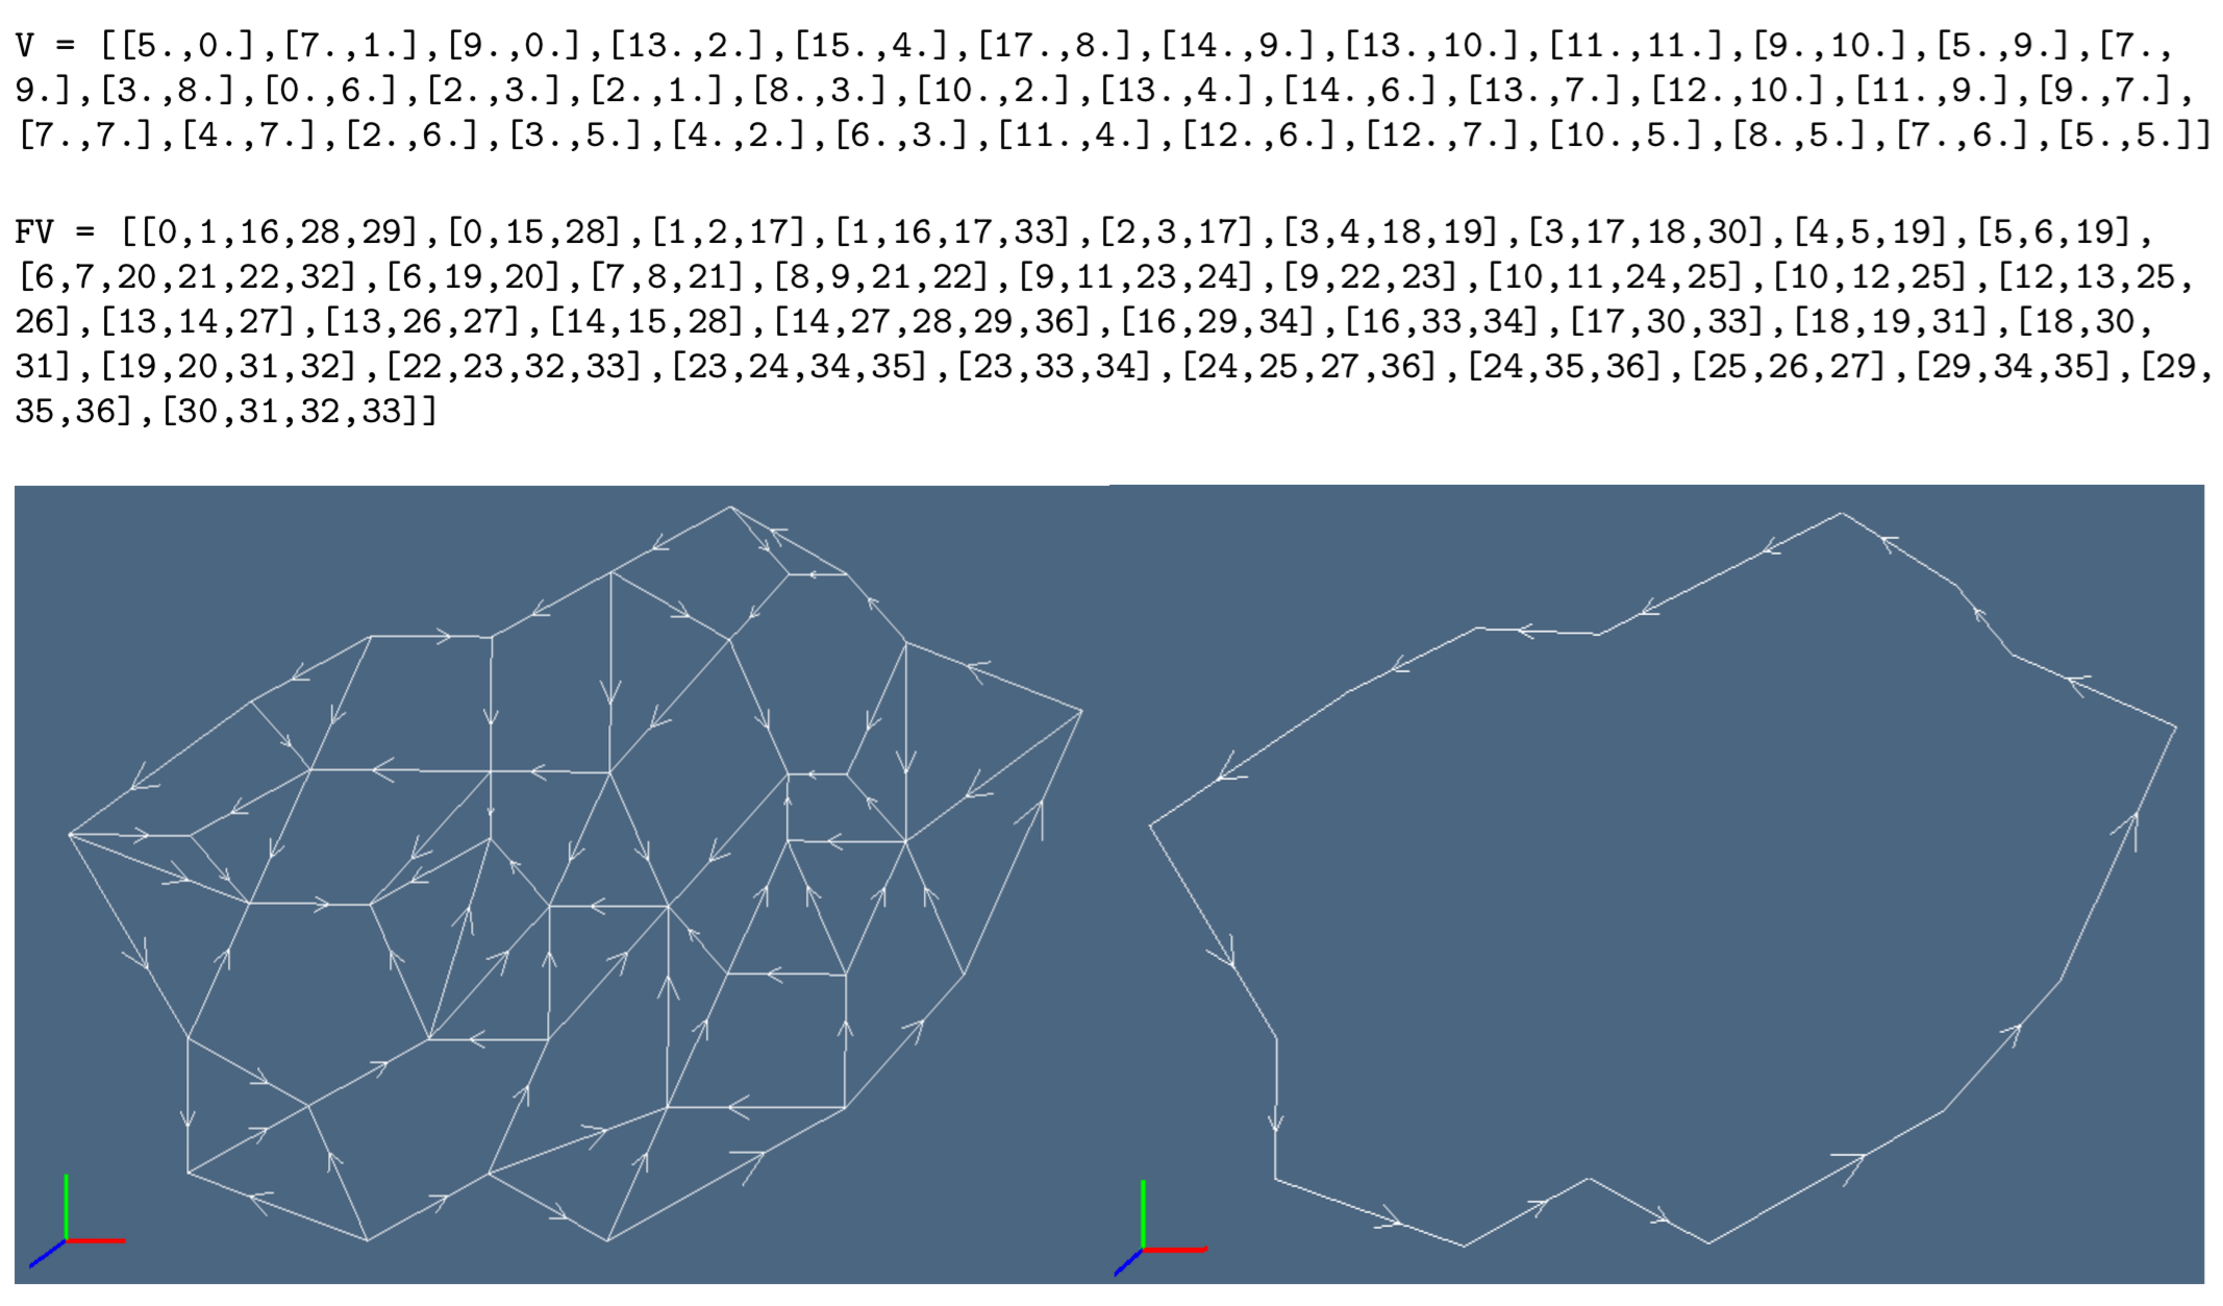
\includegraphics[width=0.5\linewidth]{images/minimum} 
 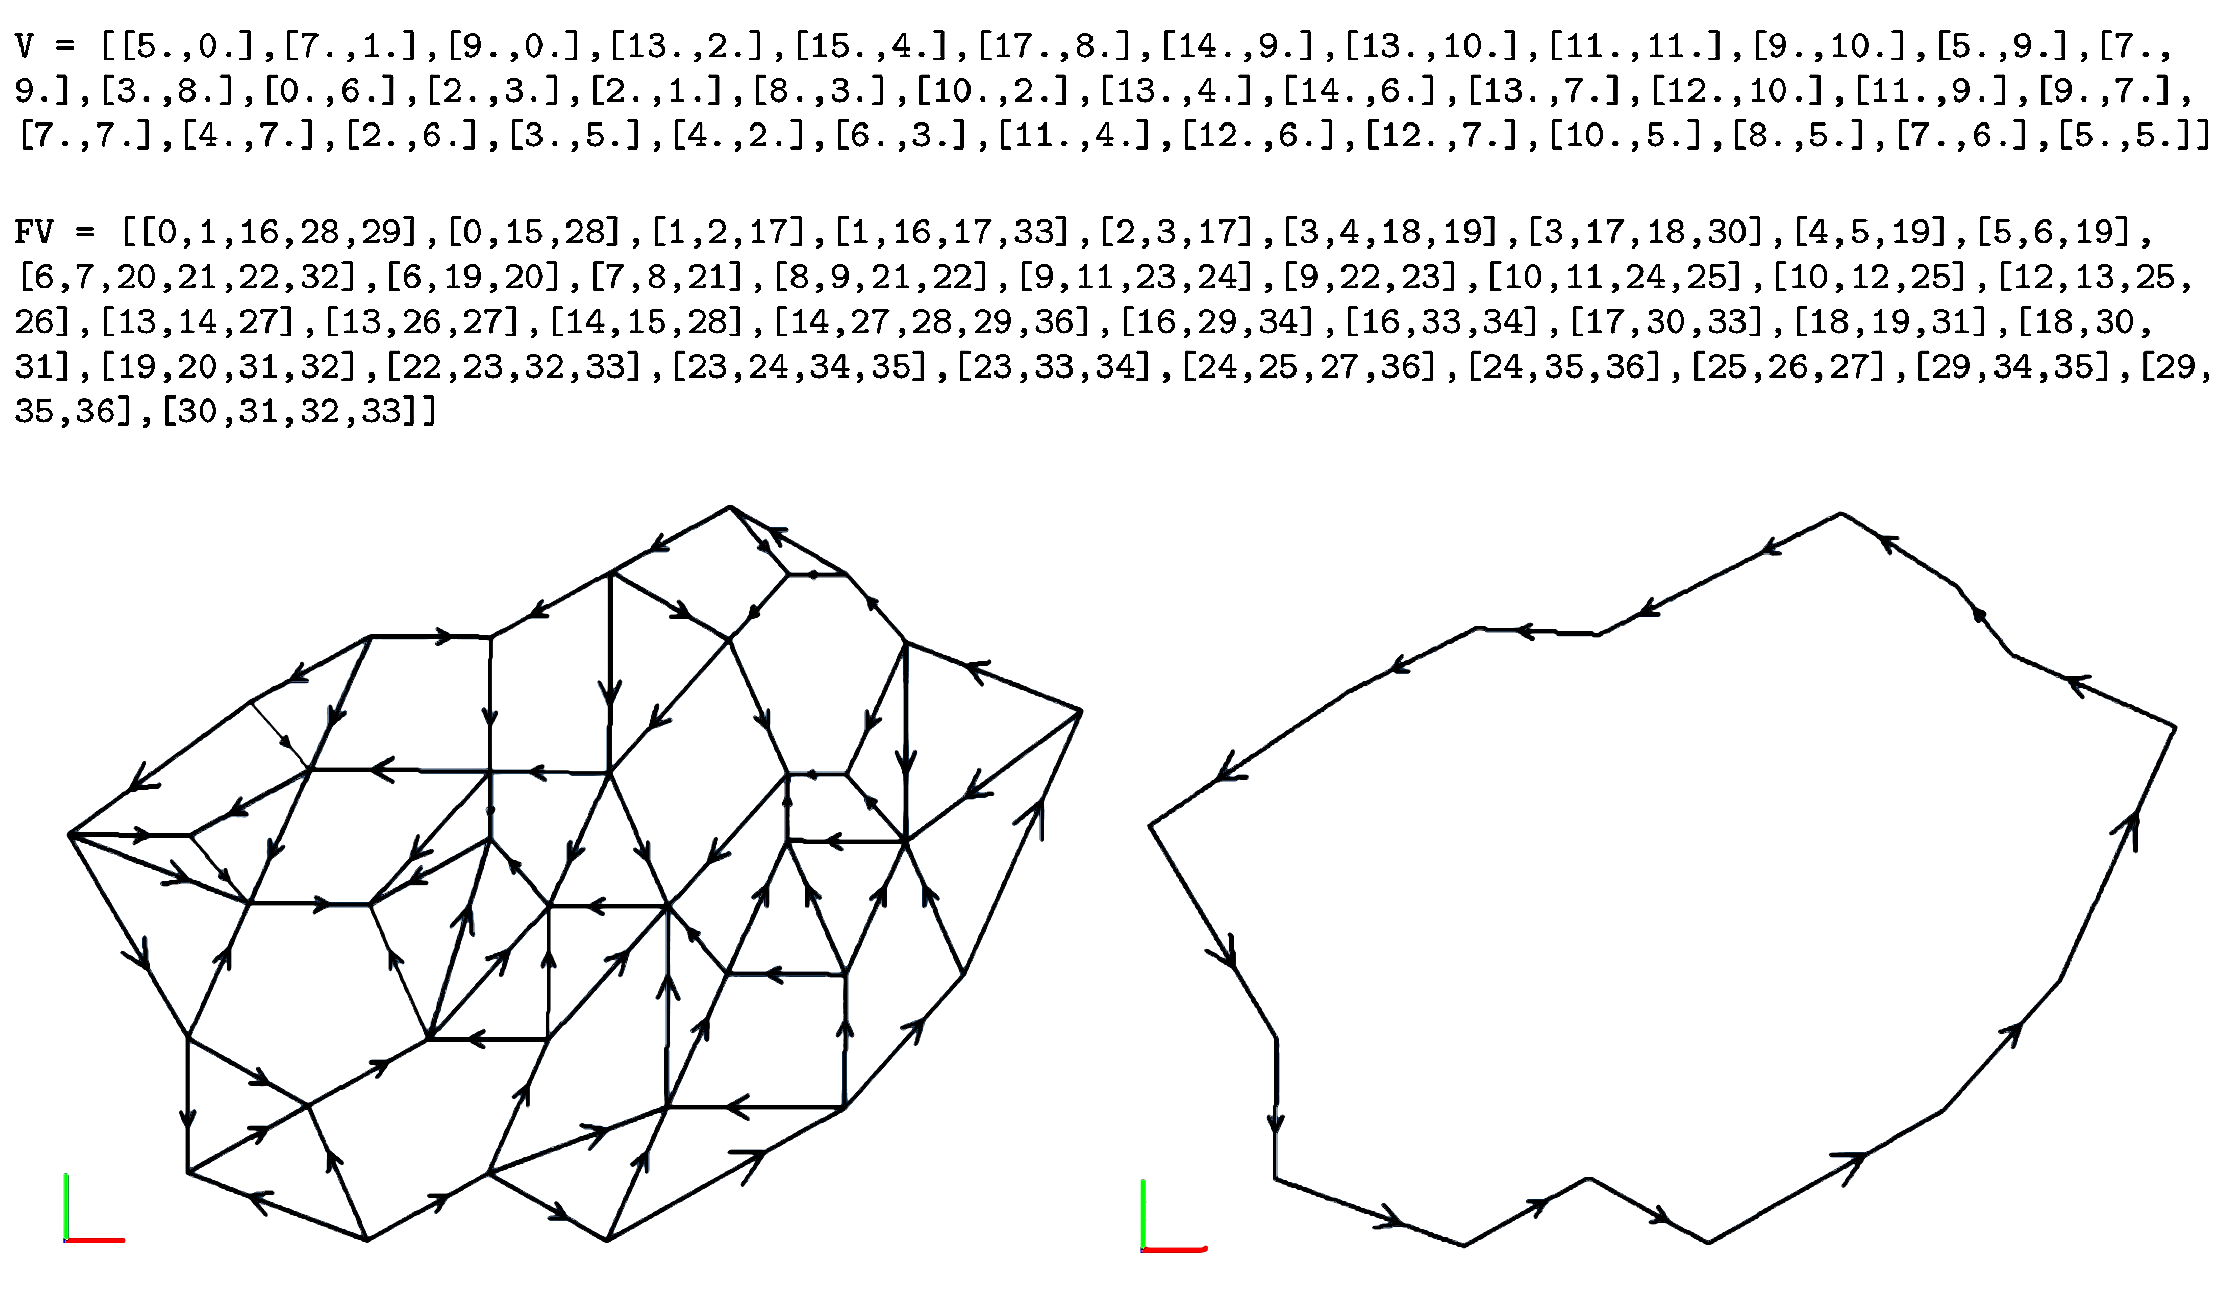
\includegraphics[width=0.5\linewidth]{images/minimum-colors-test} 
 \hfill
 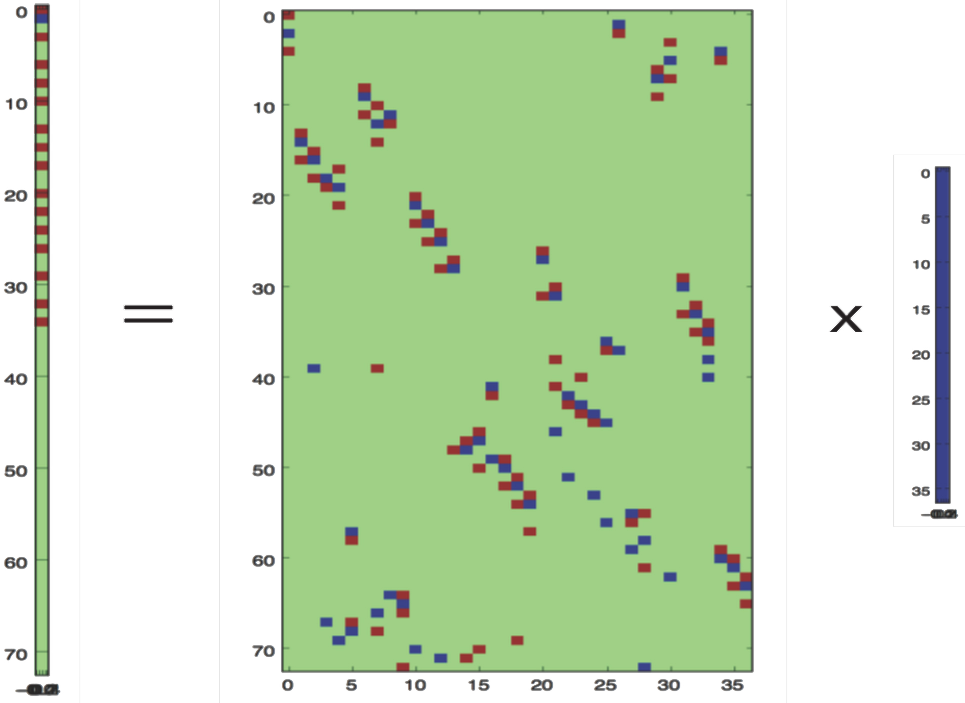
\includegraphics[width=0.4\linewidth]{images/boundary} 
 \caption{A toy example of the LAR scheme: (a) the bare minimum of data with \emph{complete} information about topology; (b) the extracted boundary; (c) the extraction method $[e] = [\partial][f]$ giving the coordinate representation (in the discrete basis of the 1-cells) of the boundary edges $[e]$ by product of the sparse boundary operator matrix $[\partial]$ times the coordinate representation $[f]$ of the 2-cells (faces), in the discrete basis of the 2-cells.}
 \label{fig:minimum}
\end{figure*}


% \begin{figure}[!h]
%  \centering
%  \begin{subfigure}[b]{\linewidth}
%  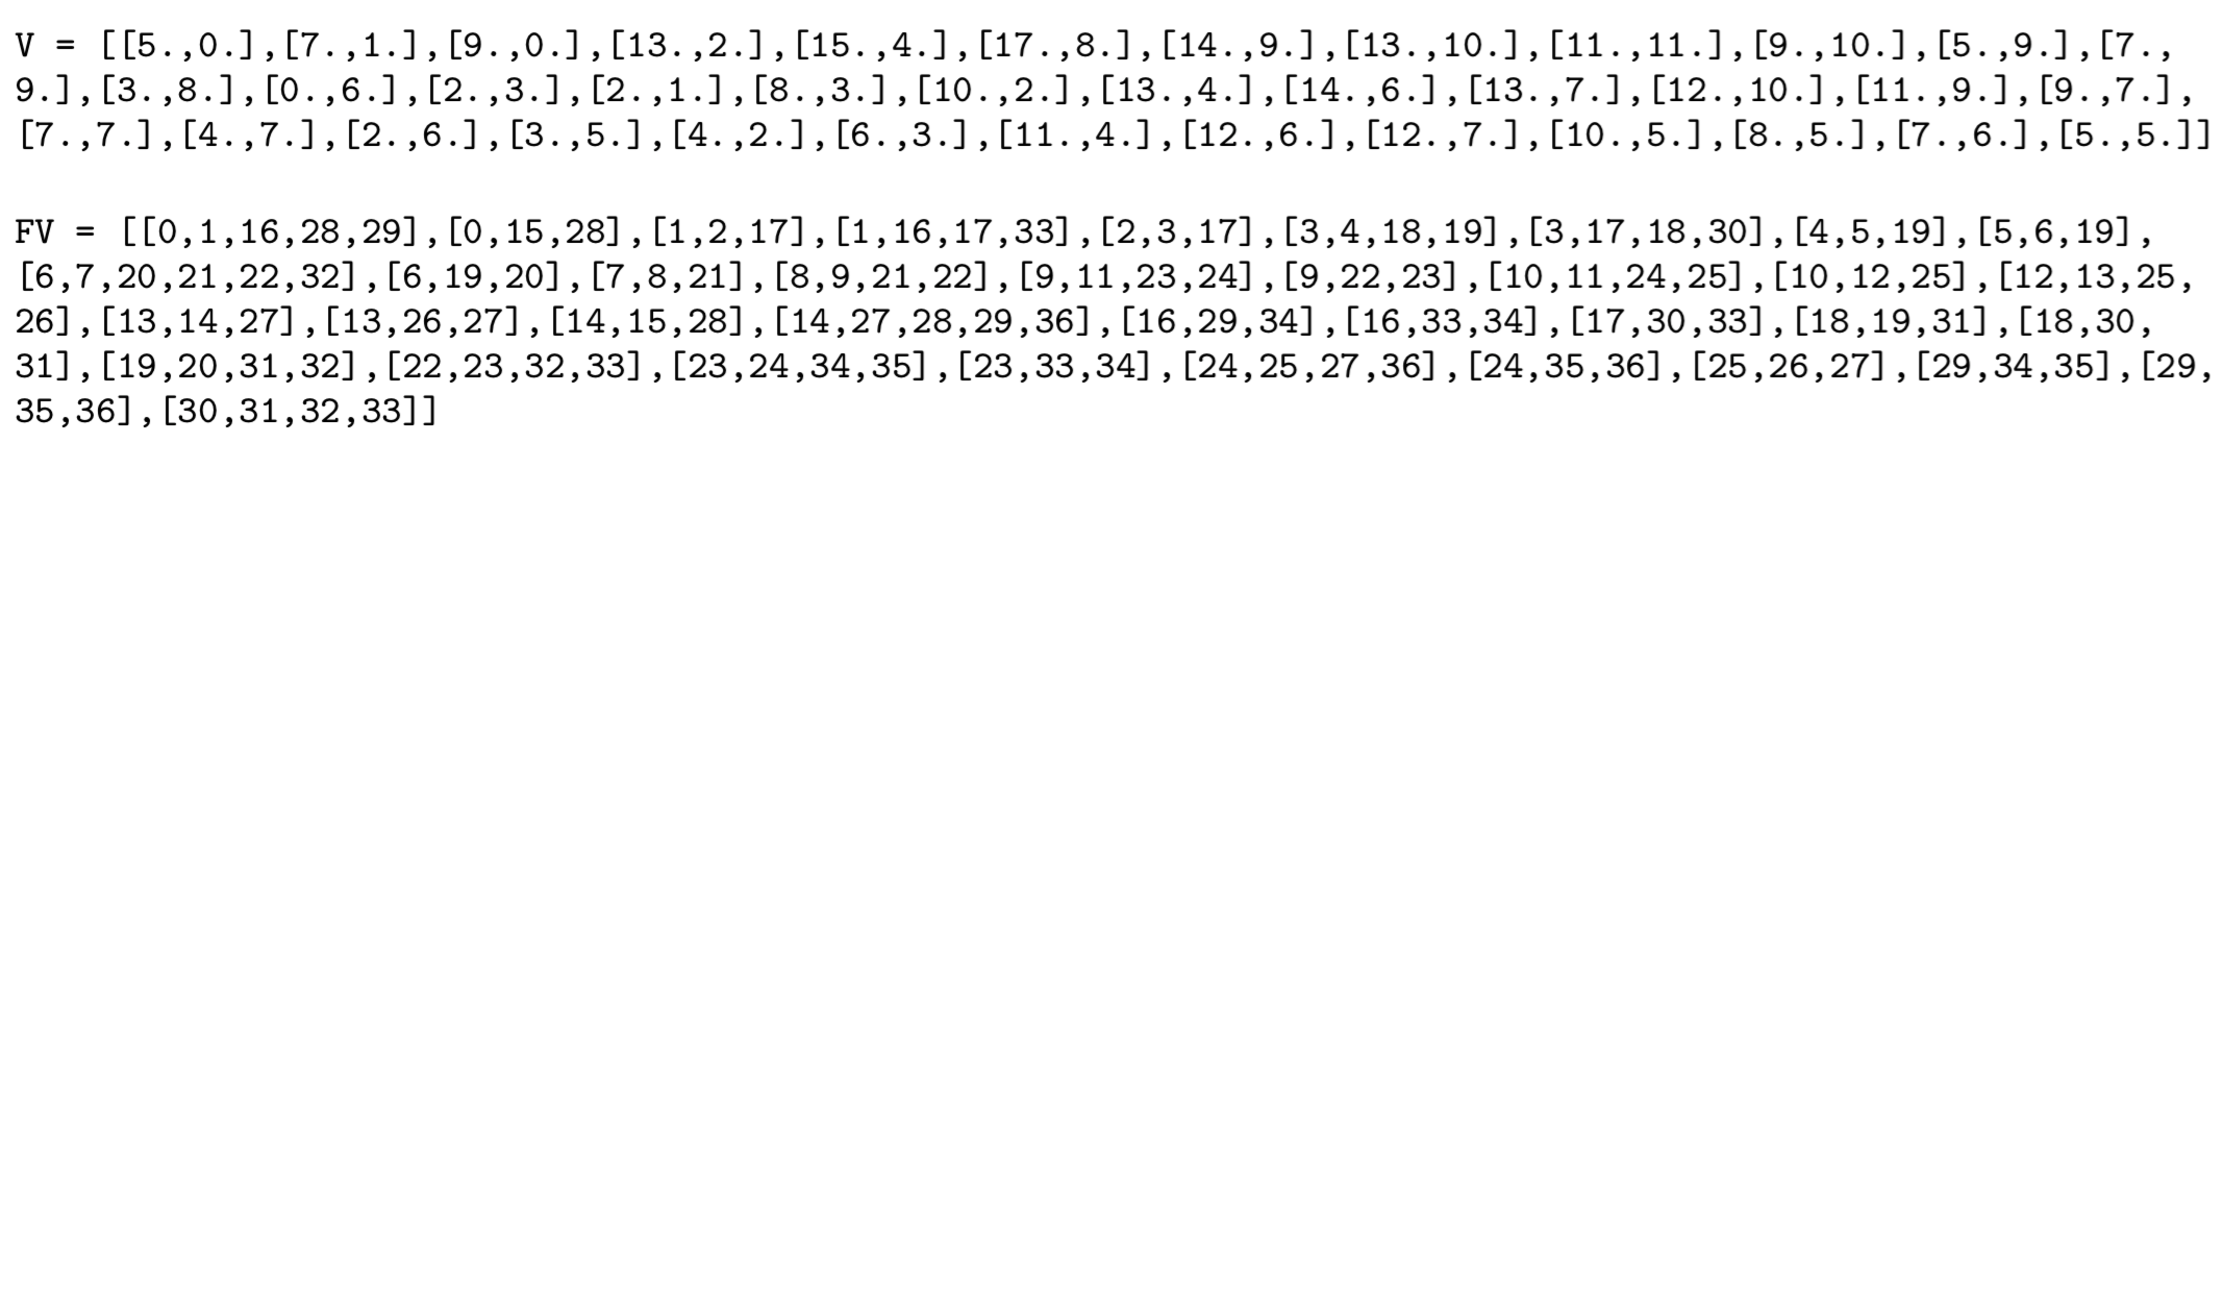
\includegraphics[width=\textwidth]{images/minimum-data}
%  \end{subfigure}
% \\
%  \begin{subfigure}[b]{0.48\linewidth}
%  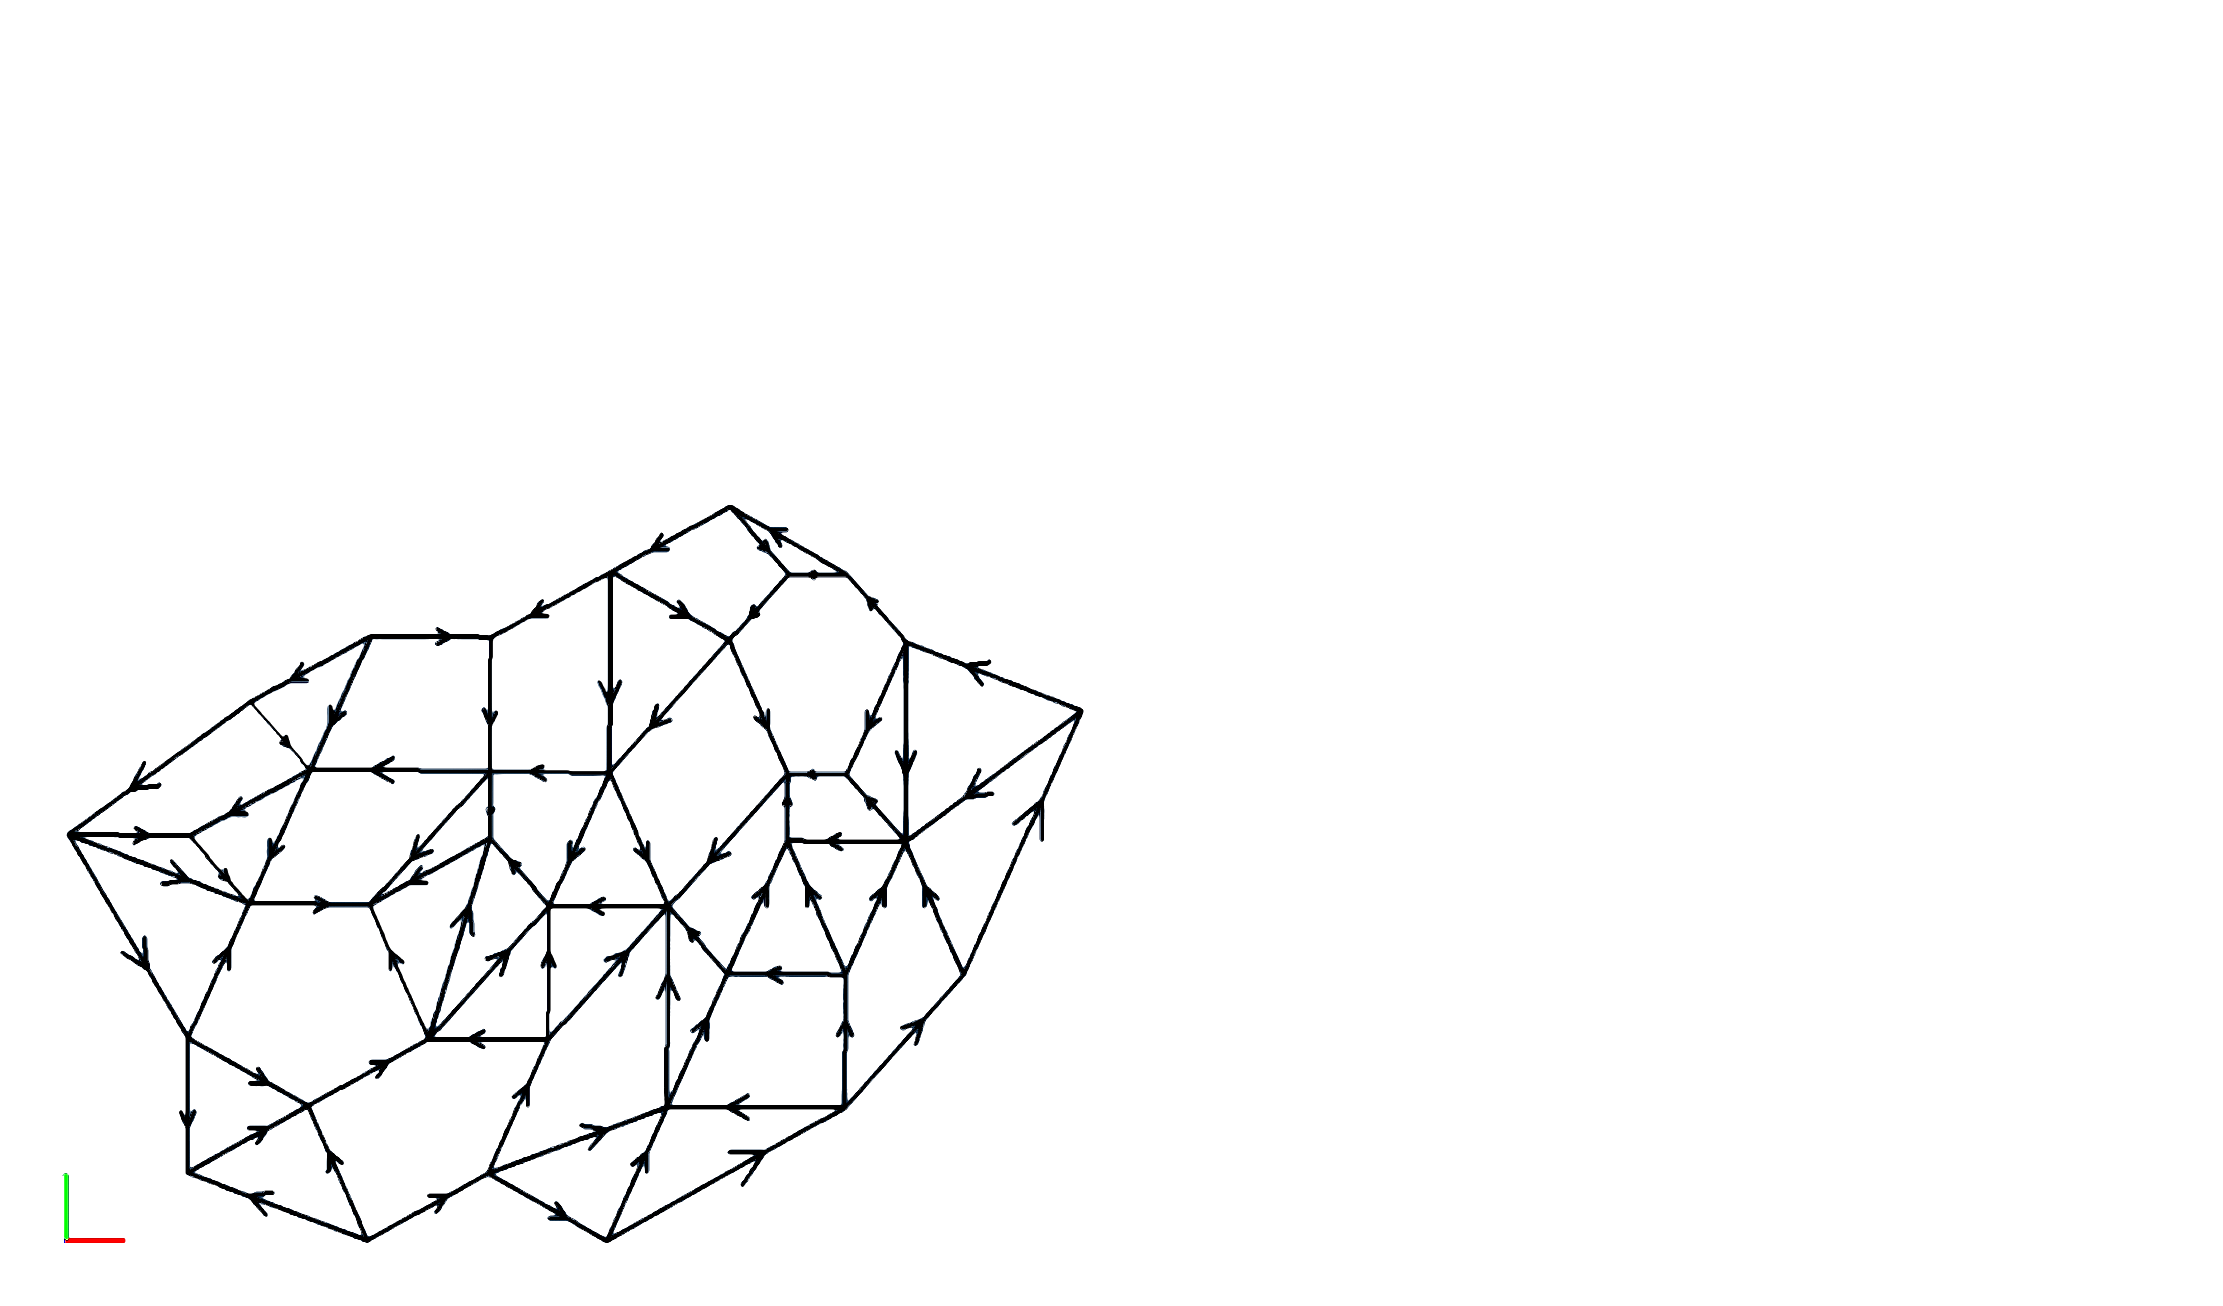
\includegraphics[width=\textwidth]{images/minimum-colors-a}
%  \caption{}
%  \vspace*{4mm}
%  \end{subfigure}
%  ~
%  \begin{subfigure}[b]{0.48\linewidth}
%  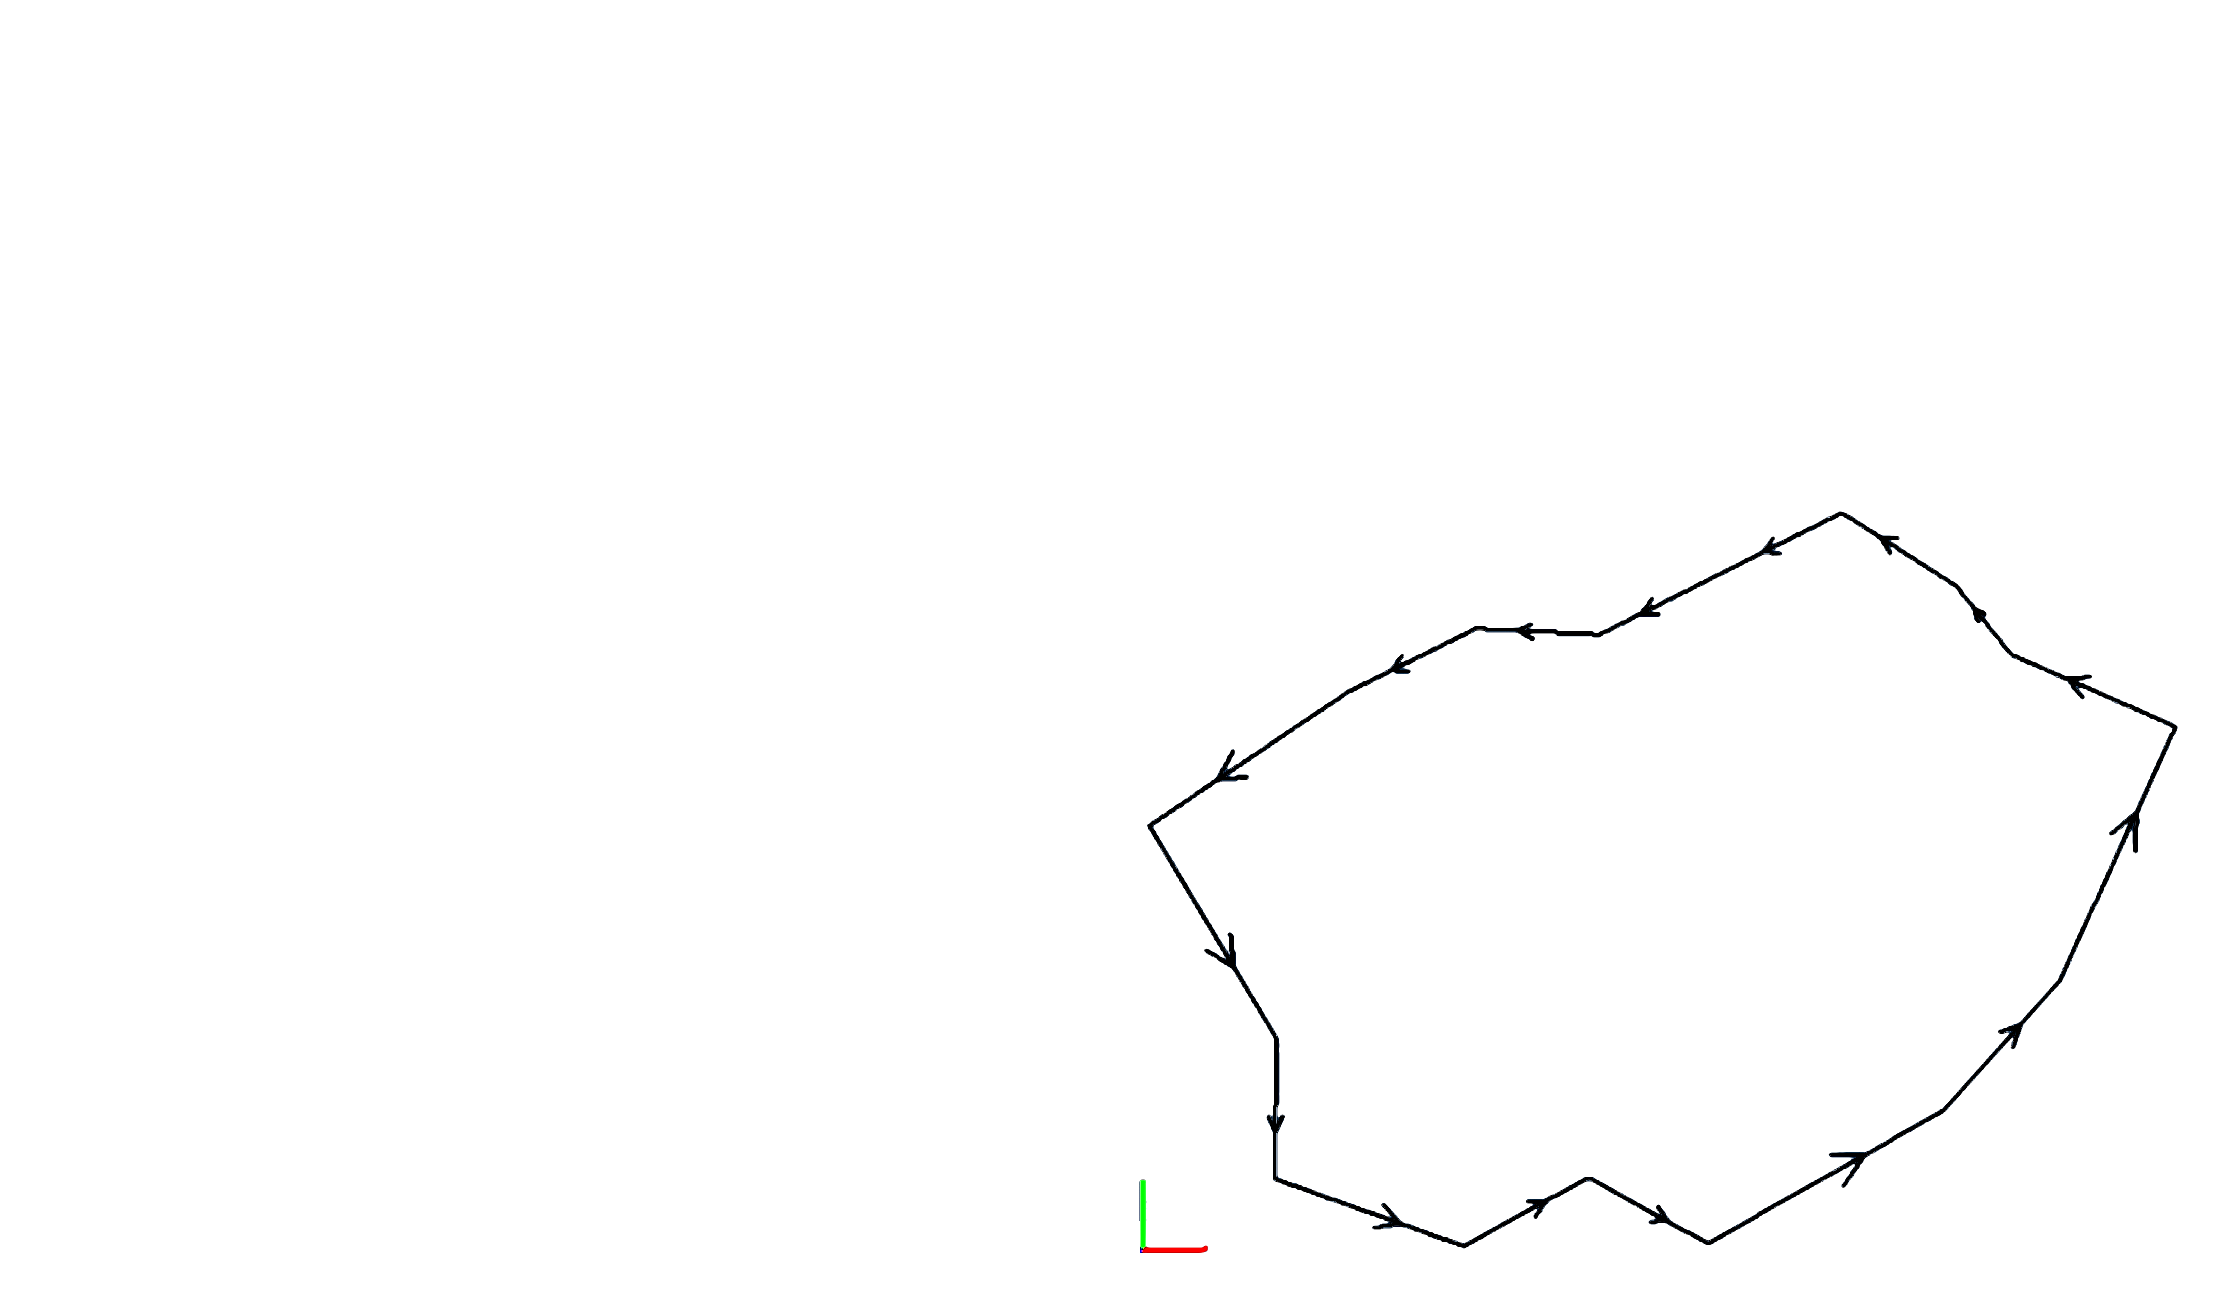
\includegraphics[width=\textwidth]{images/minimum-colors-b}
%  \caption{}
%  \vspace*{4mm}
%  \end{subfigure}
% \\
%  \begin{subfigure}[b]{0.74\linewidth}
%  \centering
%  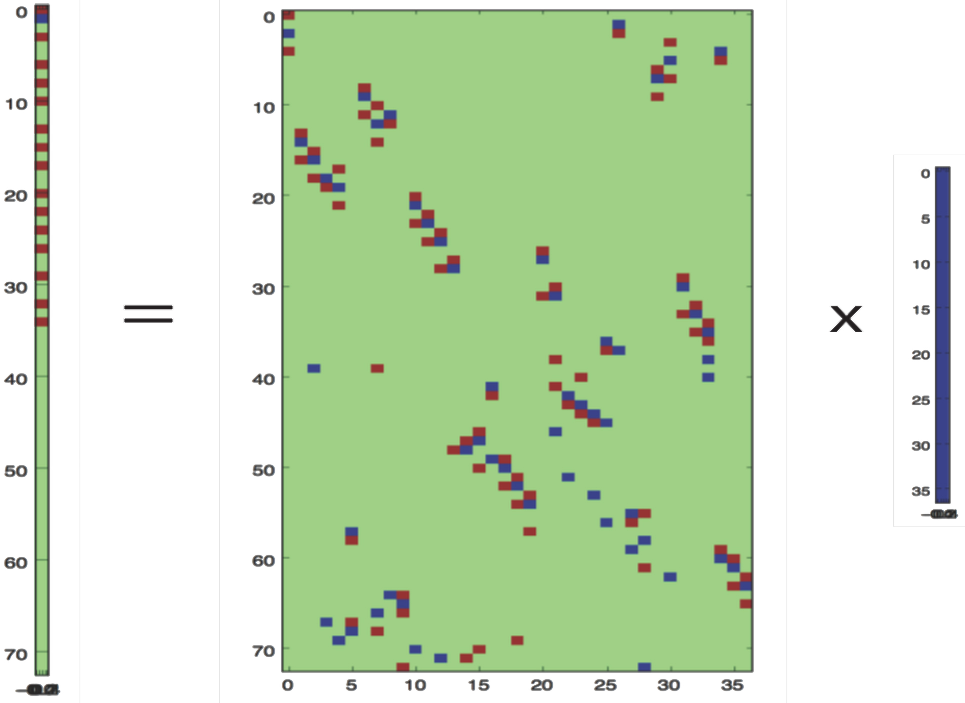
\includegraphics[width=\textwidth]{images/boundary}
%  \caption{}
%  \end{subfigure}
 
%  \caption{A toy example of the LAR scheme: (a) the bare minimum of data with \emph{complete} information about topology; (b) the extracted boundary; (c) the extraction method $[e] = [\partial][f]$ giving the coordinate representation (in the discrete basis of the 1-cells) ofthe boundary edges $[e]$ by product of the sparse boundary operator matrix $[\partial]$ times the coordinate representation $[f]$ of the 2-cells (faces), in the discrete basis of the 2-cells.}
%  \label{fig:minimum-data}
% \end{figure}

% -----------------------------------------------------------------------------


% VASTI AMBIENTI 
% MOLTI SENSORI E SISTEMI DI RILEVAZIONE DELLA POSIZIONE DIFFERENTI
% CONTINUOUS OUTDOOR-INDOOR NAVIGATION
% MONITORAGGIO DI SCENARI UNIFICATI DI INTERVENTO UOMO-MACCHINA
% PERSONALE TECNICO DEVE ESSERE GUIDATO 
% IL PASSAGGIO DA SERVER A IOT È IMMEDIATO
% MONITORAGGIO UNIFICATO DEGLI SMART OBJECTS IOT
% un ambiente indoor virtuale è l'ambiente perfetto per andare a monitorare l'IoT.

% IN QUESTO SCENARIO SI PONE IL LAVORO DESCRITTO IN QUESTO PAPER, 
% IN CUI LE NECESSIT`A DESCRITTE VENGONO AFFRONTATE PARTENDO DALLE BASI,
% OVVERO DEFINENDO UN FORMATO DI DOCUMENTO PER LA DESCRIZIONE ASTRATTA DI AMBIENTI INDOOR.
% DESCRITTO L'AMBIENTE DEVE QUINDI ESSERE POSSIBILE RICOSTRUIRE VIRTUALMENTE L'AMBIENTE
% RENDERLO LARGAMENTE ACCESSIBILE VIA WEB, E MONTARE SU QUESTA RAPPRESENTAZIONE VIRTUALE 
% LA POSSIBILIT`A DI INTERAGIRE CON GLI OGGETTI ALL'INTERNO DELL'AMBIENTE. L'INTERAZIONE DEVE CONSISTERE DA UN LATO NALLA POSSIBILIT`A DI RICEVERE INFORMAZIONI DALL'OGGETTO, MA ANCHE DI INVIARE COMANDI ALL'OGGETTP.

% SI REALIZZA IN QUESTO MODO UNO SCENARIO IN CUI UN SUPERVISORE INTERAGISCE CON L'AMBIENTE IN CUI SI MUOVE UN EXPLORER (O MANUTENTORE) POTENDO IL SUPERVISORE AVERE IMMEDIATA NOTIFICA DELLA POSIZIONE DEL MANUTENTORE, E AVENDO UN QUADRO COMPLETO FORNITO DAGLI OGGETTI SMART PRESENTI NELL'AMBIENTE REALE ASSIEME ALL'EXPLORER.

% D'ALTRA PARTE PER GRANDI SPAZI ANCHE L'EXPLORER PUO ESSERE SUPPORTATO DAL SISTEMA CHE AVENDO COMPLETA CONOSCENZA DELLA TOPOLOGIA E DELLA GEOMETRIA DELL'AMBIENTE, NONCHE DEGLI OGGETTI IN ESSO CONTENUTI, POSSIEDE TUTTE LE INFORMAZIONI NECESSARIE PER GUIDARE L'EXPLORER ATTRAVERSO L'AMBIENTE.

% NULLA IMPEDISCE DI MIXARE LE NECESSITÀ DI EXPLORER E SUPERVISOR, REALIZZANDO UN EXPLORER CHE NAVIGA NELL'AMBIENTE REALE ED IN ESSO RICEVE INFORMAZIONE E A CONTEMPO PUÒ INVIARE COMANDI AGLI SMART OBJECT INTORNO A SE.


\section{Related work}\label{related-work}

Research on the cartographic representation of indoor environments is
extensive and heterogeneous with respect to the strategies
applied. Different information sources are used, and accuracy of the
produced solution depends on the adopted approach. In some cases the
information is obtained with automatic or semi-automatic processing of files
that describe the architectural structure of a building, such as BIM (Building Information Modeling)~\cite{Eastman:2008:BHG:1796500} and/or IFC (Industry Foundation Classes) that describe a building project \cite{6816739}. Image processing is also used to
extract topological information from floor plan images \cite{6878152}. In
other works, building information and descriptive parameters are redefined
from scratch \cite{6418876}. Such approaches suffer from the non appropriateness of
their representative formats: images contain poor information and CAD
files are not designed for this kind of use. 

A recurring theme among the use
of cartographic information is \emph{indoor navigation}
\cite{6878152,6418876,6816739}. The proposed approaches are very different in
this case too, and based on several strategies with some basic elements in
common. An often adopted solution is based on the representation of the
routing information as a graph, having a node for each room and an edge for
each pair of connected rooms. In some cases the edges are weighted in
function of euclidean distance. The detail level of the graph, and hence the
effective usefulness of the calculated paths, can vary depending on the
technique and the design choices applied, but in general most of the proposed
solutions retrieve information only from architectural structure. 

A subject related to navigation is the \emph{location of users}. To locate the exact position of a user inside a
building, the currently most applied techniques are based on fingerprinting and
triangulation of radio signals (Wi-Fi, Bluetooth, LTE, etc.) flanked by more
original solutions based, for example, on image recognition \cite{6815564}.
User tracking issue is faced with solutions that range from the clever
utilization of inertial tracking sensors embedded in many smartphones
\cite{6815564} to the adoption of ad hoc devices \cite{6878152}.

The actual ``de-facto'' standard in terms of geospatial data representation is
the \emph{GeoJSON} format, which can be easily used for any type of geographical
annotation. In some cases it has been slightly adapted to be used in indoor
environments: it is the case of the \emph{IndoorJSON} format.

\subsection{The GeoJSON format}\label{the-geojson-format}

\emph{GeoJSON} is a geospatial data interchange format based on JSON, suitable for a
geometrical encoding of various geographic data structures. As opposed to GIS
formats, GeoJSON is an open standard. Positions need to be expressed in
geographical coordinates (usually WGS84).

GeoJSON supports some geometric primitives, including: {\tt Point},
{\tt Line\-String}, {\tt Polygon}, {\tt MultiPoint},
{\tt MultiLineString}, and {\tt MultiPolygon}. Lists of geometries are
represented by a {\tt GeometryCollection}. Geometries with additional
properties are {\tt Feature} objects. Lists of {\tt Feature} are
represented by a {\tt FeatureCollection}.

A single {\tt Feature} is composed essentially by two mandatory fields:
{\tt geometry}, which describes the object geometry accordingly to the
previously recalled primitives, and {\tt properties} which contains
additional information about the {\tt Feature}.

In GeoJSON it is possible to define complex shapes through the composition of simpler
 objects. Mainly due to its simplicity, GeoJSON is widely used and
deeply integrated in several applications and services.

\subsection{The IndoorJSON format}\label{experiences-on-indoor-json}

\emph{IndoorJSON} is a GeoJSON variant defined and used by \emph{indoor.io}, a
Finnish company devoted to indoor environment mapping. IndoorJSON is compliant
with GeoJSON syntax, and it may consist of any number of {\tt Features}
and/or {\tt FeatureCollections}. All {\tt Features} are interpreted
similarly regardless of their grouping into nested
{\tt FeatureCollections}. IndoorJSON supports all GeoJSON geometry types.

Some particular properties are used to correctly define the indoor elements:

\begin{itemize}
\itemsep1pt\parskip0pt\parsep0pt
\item
 {\tt level}: describes which level contains the feature;
\item
 {\tt geomType}: identifies the object's
 category, useful during the visualization
 process.
\end{itemize}

There are some additional but not mandatories properties, useful for
the indoor representation:

\begin{itemize}
\itemsep1pt\parskip0pt\parsep0pt
\item
 {\tt accessible}: describes if an element is walkable or not;
\item
 {\tt connector}: defines if the element is a connection between two
 levels;
\item
 {\tt direction}: describes the direction of the connection (both
 ways, only up, only down);
\end{itemize}

A syntax validator is provided by \emph{indoor.io}, but the commercial nature
of this project limits the number of tools available to deal with this
format.



\section{Advances on cartographic\\ document formats}\label{advances-on-cartographic-document-format}
\label{advances}

The focus of this work is the definition of a novel format of cartographic
documents along with the software ecosystem rooted on it. A simple but
effective algorithm to find indoor valid routes is also provided. The {HIJSON}
(\textbf{H}ierarchical \textbf{I}ndoor \textbf{JSON}, this is the name chosen
for the format) and the accompanying software framework aim to realize a
mapping of indoor real spaces with a virtual interactive web environment. The
HIJSON is based upon ideas and design principles collected from previous
formats and identifies four critical improvements with respect to them: it
exposes a \emph{hierarchical structure}, uses \emph{metric local coordinate
system} \emph{imports external hyperlinked geometric models} and accepts \emph{semantic
extensions}. 
% Furthermore, geometrical  and topological data are conveniently imported and represented via LAR, an advanced  representation scheme, allowing to deal with \emph{hyperlinked geometric models}.

\subsection{Hierarchical structure}\label{hierarchical-structure}

The HIJSON format allows for hierarchical description of indoor spaces. The
introduction of a hierarchical structure establishes a parent-child relation
between entities of the model, reflecting a container-contained relationship.
This direclty implies a neater representation than the plain linear structure
adopted by GeoJSON, being a perfect analogy of objects contained (i.e.
placed) into spaces.

In addition, more organized arrangement is allowed by logical (or even
physical) grouping: concepts like building wings, sections, stories,
departemens, etc. can be introduced to reflect into the document structure
logical or physical real divisions, categories or relashionships.

Hierarchical structures are common in computer graphics since they are used as
scenegraphs. This accordance of underlying structures really simplify 3D
render algorithms of HIJSON documented environments.

Furthermore the container-contained relation enables to use local reference system.

\subsection{Metric local coordinate system}\label{metric-local-coordinate-system}

Supported by the hierarchical underlying structure, the HJSON document format allows 
for the use of local coordinate system. This means that the shape of all elements can 
be convenient modelled using local coordinate and than placed in the right position 
with respect to the position of the parent (or container) element applying a 
translation and a rotation vector.

Another substantial advantage is represented by the adoption of a metric reference, 
consequently simplifying the compilation of the document, however it is, 
manual or aided by software tools.

The HIJSON document format is specially designed to guarantee the user to be routed seamlessly 
from outdoor to indoor and vice versa. Even though indoor geometries are inputted in a metric 
local continuous outdoor-indoor navigation is ensured via the definition of a processing pipeline
detailed in the following.

\subsection{Hyperlinked geometric models}\label{optional-lar}

A HIJSON document may further import external geometric models---either of the buildings itself or the interior furniture or devices---that are topologically complete (in the sense of solid modeling~\cite{Requicha:1980:RRS:356827.356833}) and very compact. 
Such models coming from a source outside the document are acquired by linking JSON files that contain a Linear Algebraic Representation (LAR) of topology and geometry, to be expanded for visualization or interaction at any useful level of detail. 

The LAR scheme~\cite{Dicarlo:2014:TNL:2543138.2543294} is characterised by a very large domain, including architecture, building and construction~\cite{paoluzziMS:2014}, 2D and 3D engineering meshes, non-manifold geometric and solid models and meshes, and high-resolution 3D images~\cite{cadanda:2015}. This scheme uses the set of \emph{Combinatorial Cellular Complexes} (CCC) as mathematical domain
\cite{Basak:2010}, and various compressed representations of \emph{sparse matrices} \cite{gemmexp} as codomain. 

Since LAR provides a complete representation of the topology of the represented space,
the matrix $[\partial_d]$ of the boundary operator shall be used to compute the coordinate representation $[c]$ of the \emph{boundary} chain of \emph{any subset} $c$ of cells, though \emph{a single} operation of SpMV multiplication \cite{gemmexp} between the \texttt{CSR} (Compressed Sparse Row) representation of $[\partial]$ and the \texttt{CSC} (Compressed Sparse Column) representation of the $[c]$ chain, resulting in very efficient computations on modern hardware, even mobile.

The expansion of a LAR model, to be considered as a general-purpose graphic primitive, may be executed on either the server or the supervisor client of the HIJSON Web Toolkit architecture (see Section~\ref{server-architecture}), or even on the \emph{Explorer} client, depending on the size and the locality of the model to be expanded.

% \begin{figure}[htbp] % figure placement: here, top, bottom, or page
% \centering
% \includegraphics[width=\linewidth]{images/sogei} 
% \caption{Office building: (a) the schematic plan; (b) the simplified 3D model generated for testing on the field the in-door mapping project described in this paper.}
% \label{fig:sogei}
% \end{figure}

\begin{figure}[!h]
 \centering
 \begin{subfigure}[b]{0.48\linewidth}
 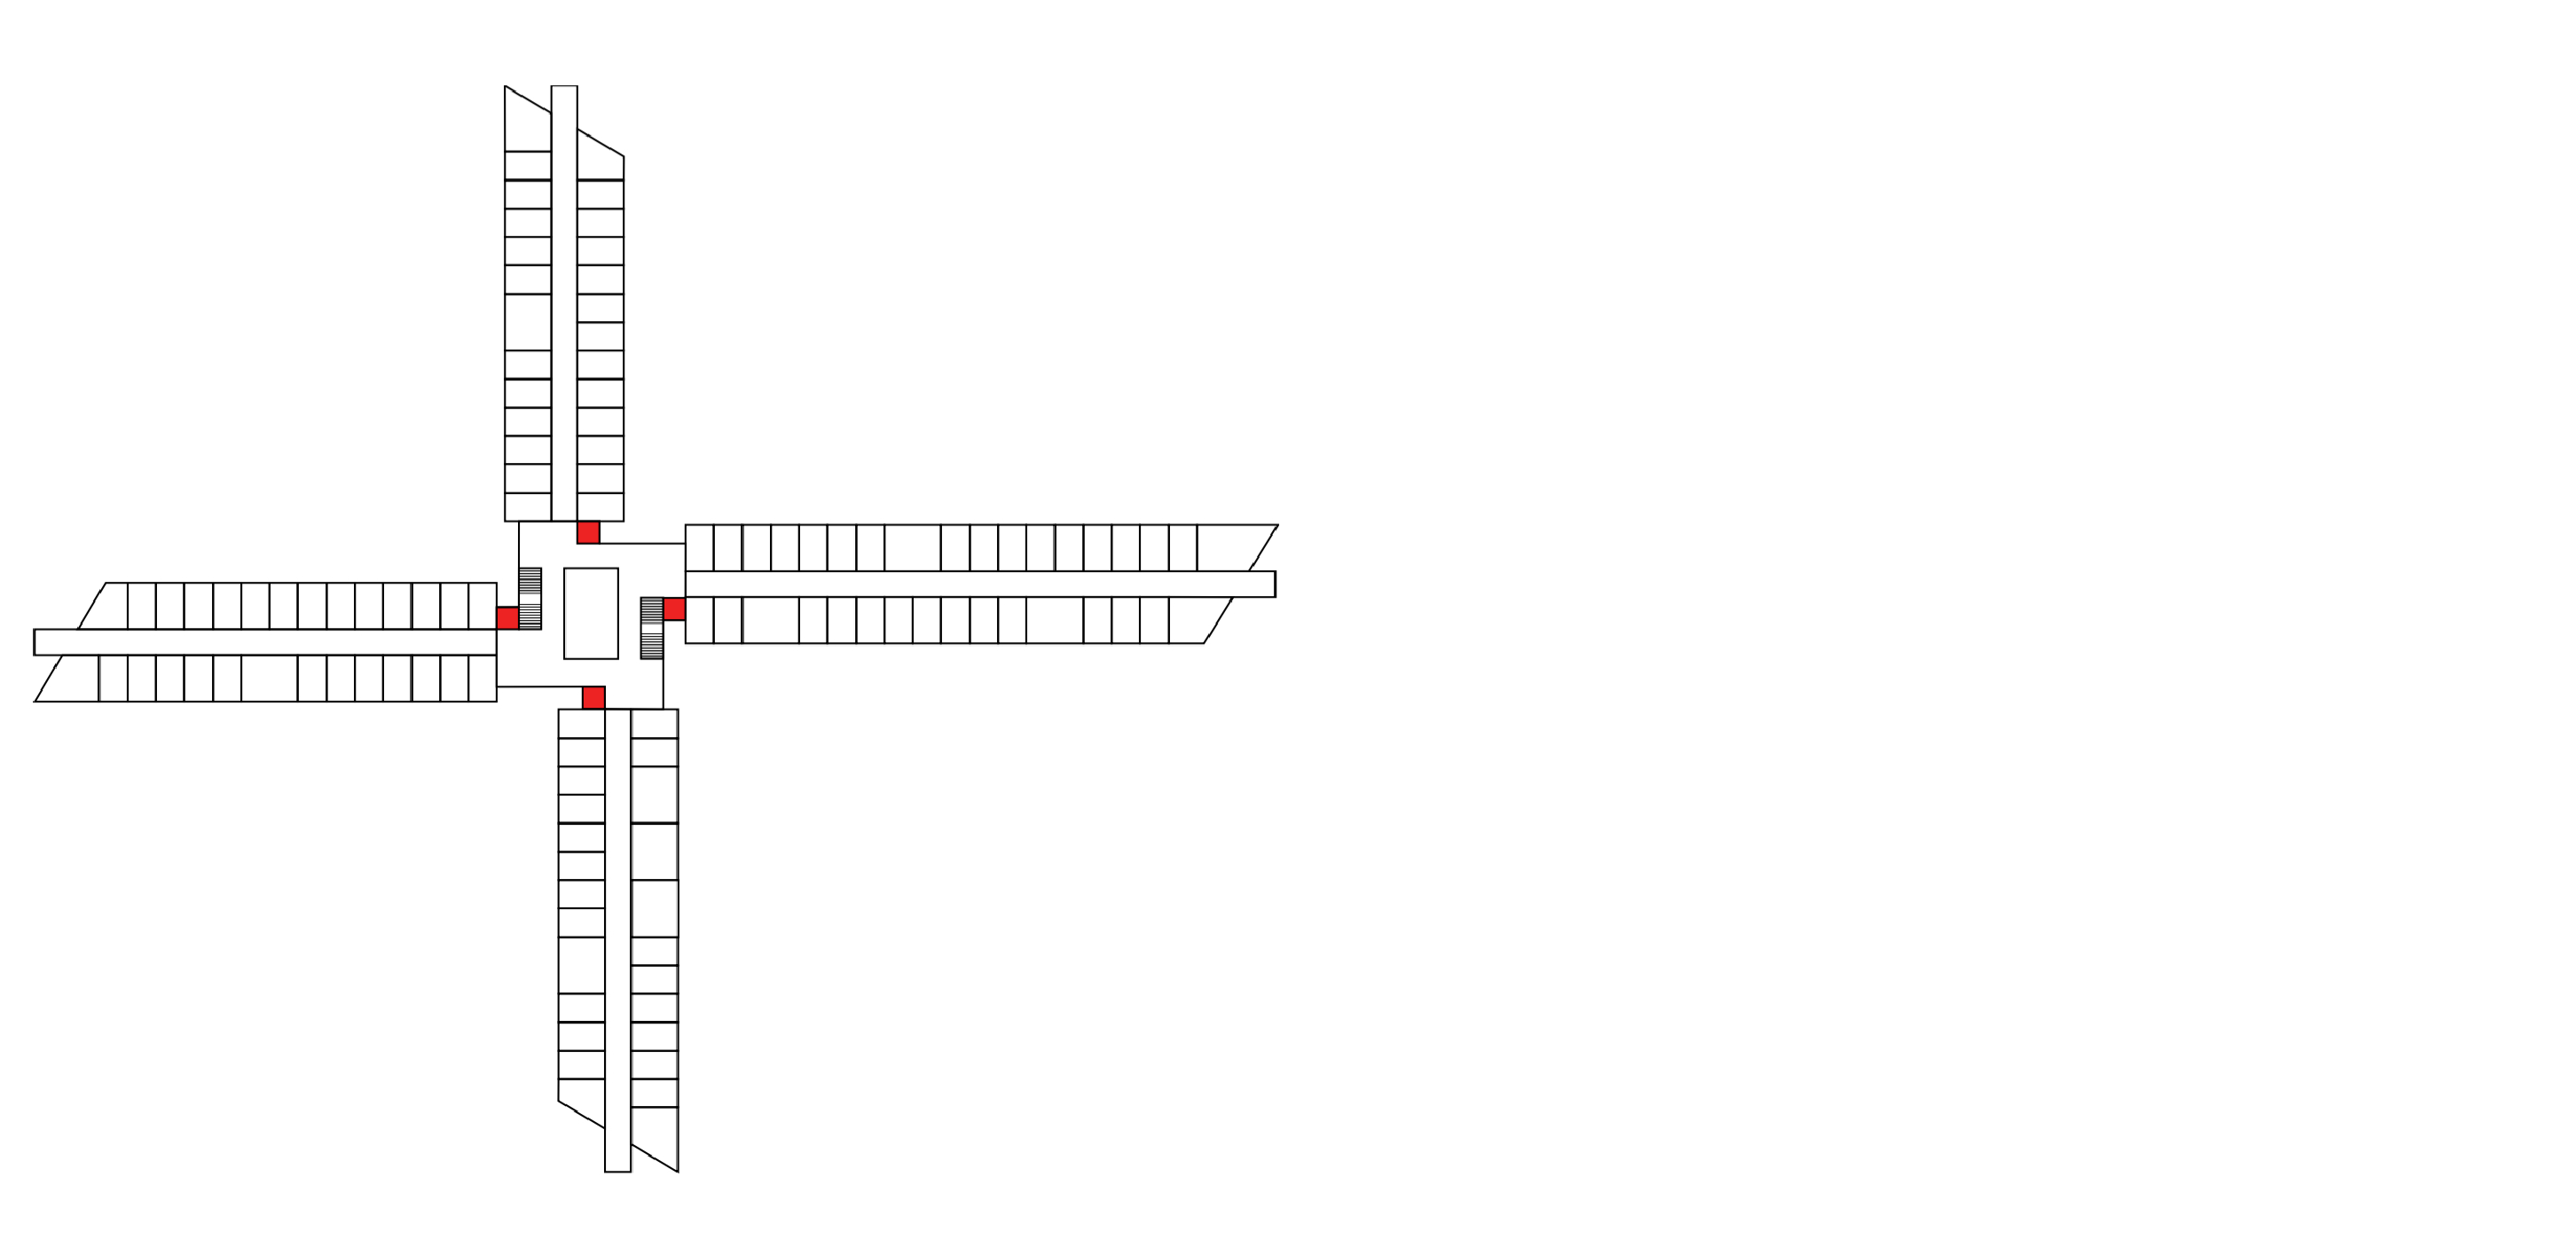
\includegraphics[width=\textwidth]{images/sogei-a} 
 \caption{}
 \label{fig:sogei-a}
 \end{subfigure}
 ~
 \begin{subfigure}[b]{0.48\linewidth}
 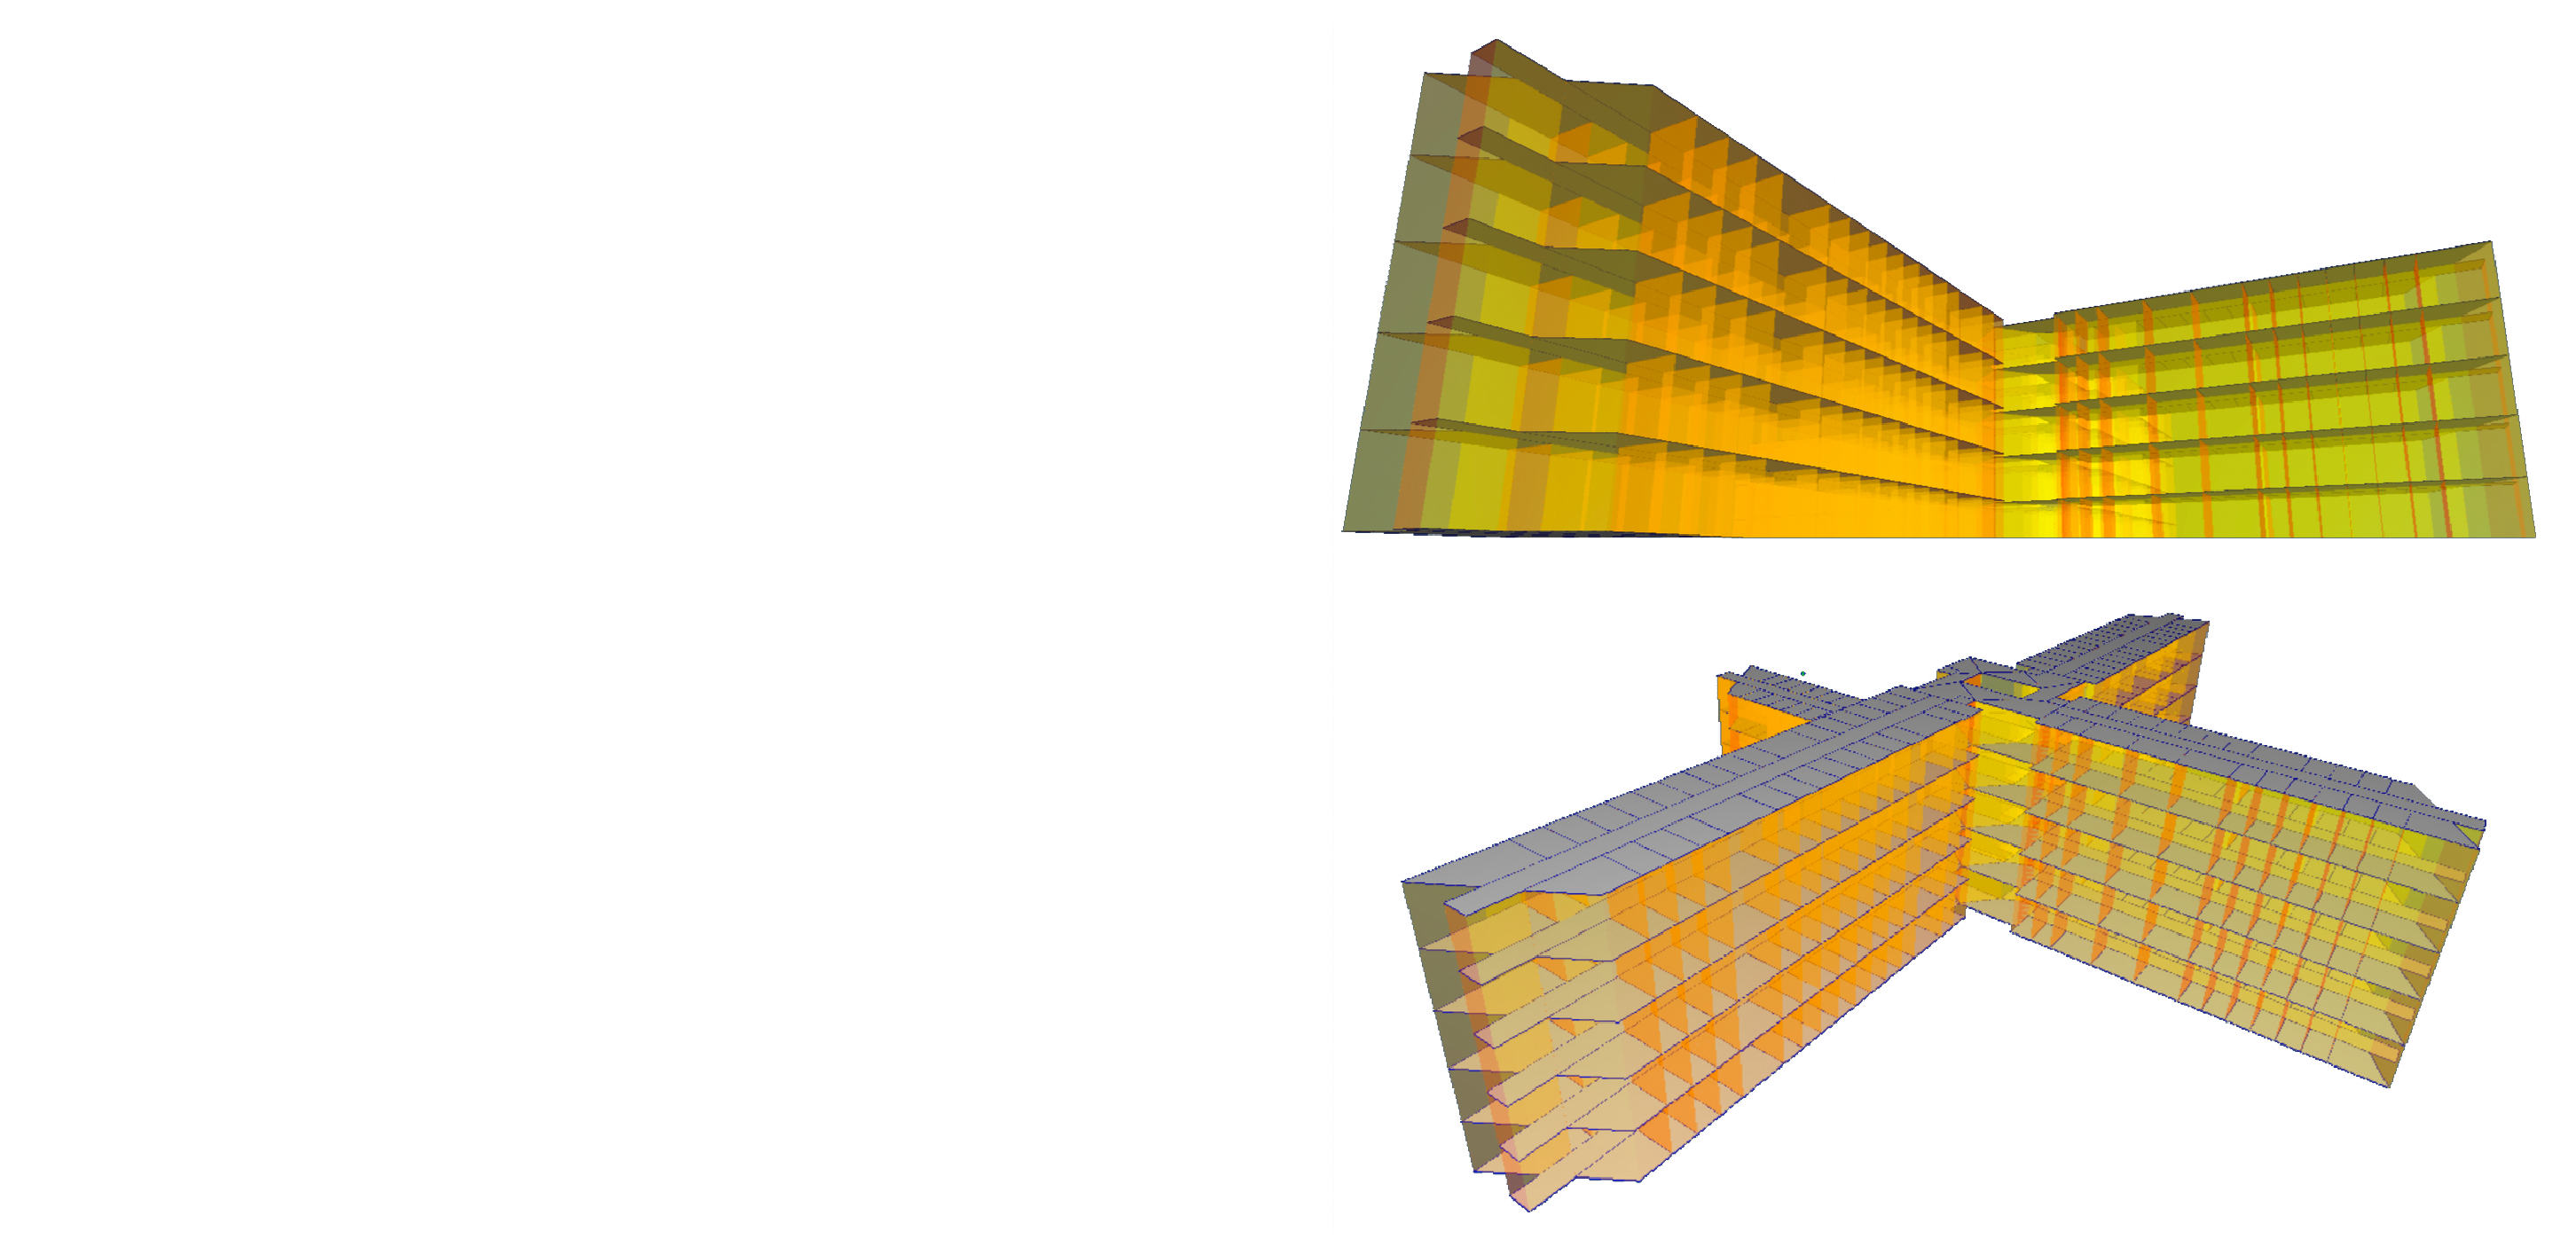
\includegraphics[width=\textwidth]{images/sogei-b}
 \caption{}
 \label{fig:sogei-b}
 \end{subfigure}
 
 \caption{Office building: 
 (a) the schematic plan; 
 (b) the simplified 3D model generated for testing on the field 
 the in-door mapping project described in this paper.
 }
 \label{fig:sogei}
\end{figure}

\subsection{Semantic extensions}\label{semantic-extensions}

Semantic extensions make the HIJSON format extendible and customizable, that
is, able to adequately respond to any need of objects representation. To define a
semantic extension means to allow the HIJSON document to model an object
previously not covered, or even to modify the behaviour of a comprised one.
Semantic extensions are to be defined both as HIJSON format syntyax and as
HIJSON Toolk source code. In particular it is necessary to define respectively
a new HIJSON Element and a new HIJSON Class, as specified below.




\section{HIJSON structure and syntax}\label{hijson-syntax}

The HIJSON document is composed by a configuration section, followed by one or more {\tt FeatureCollections}, containing the actual data.

Listing~\ref{lst:hijson-example} shows a simplified HIJSON document, devoid of punctual details, to make clear to the reader the overall document structure.

\vfill

\begin{lstlisting}[language=json, label={lst:hijson-example}, captionpos=b, caption=Example of HIJSON document.]
{
  "config": {
    // ...
  },
  "data": [
    // ...
    {
      "id": "architecture",
      "type": "FeatureCollection",
      "features": [
        // ...
      ] 
    },
    {
      "id": "furniture_1",
      "type": "FeatureCollection",
      "features": [
        // ...
      ] 
    },
    // ...
  ]
}
\end{lstlisting}


The configuration includes parameters and settings needed for building representation in the form of a JSON Object. One of the core information in this section is defined by the correspondence between three points of the local coordinate system and three points of the real world, expressed in geographical coordinates. This is needed to ensure a seamlessly passage from local to geographical coordinate system and vice versa.

After the configuration part, the document includes a list of {\tt FeatureCollection}. An example
of {\tt FeatureCollection} is given in listing~\ref{lst:feature-collection-example}.


\begin{lstlisting}[language=json, label={lst:feature-collection-example}, captionpos=b,  caption=Example of {\tt FeatureCollection}.]
{
  "id": "architecture",
  "type": "FeatureCollection",
  "features": [
    // ...
    {
      "type": "Feature",
      "id": "room_0.1",
      "geometry": {
        "type": "Polygon",
        "coordinates": [
          [ [0, 0], [11, 0], [11, 19], [0, 19] ]
        ]
      },
      "properties": {
        "class": "room",
        "parent": "level_0",
        "description": "Office of Mr. Smith",
        "tVector": [10, 20, 0],
        "rVector": [0, 0, 90]
      }
    },
    // ...
  ]
}
\end{lstlisting}

Each element of the list is given in the form of a GeoJSON {\tt
FeatureCollection}, that contains an arbitrary  number of HIJSON Elements.
Each {\tt FeatureCollection} imposes a logical relationship that can be used
to group together related HIJSON Elements. Since  HIJSON Elements adhere to
the GeoJSON format, each {\tt FeatureCollectio}n results compliant with GeoJSON
syntax and then accepted by any GeoJSON validator. As detailed below, the
HIJSON format  introduces some additional rules that allow the adoption of
this format for indoor representation.


\subsection{HIJSON Element}

Dealing with indoor environments, there are essentially two classes of objects
that is necessary to represent. They are (a) architectural elements, like a
room, a corridor, a wall, etc. and (b) furnishings, intended in a broad sense,
such as to contain both furniture, like a desk or a chair, and/or ``smart objects'',
like an IP-cam or a connected thermostat.

A HIJSON Element defines a GeoJSON compliant syntax to describe both geometry and properties of
an object. It represents the atomic component of a HIJSON document. 
It would be a best practice to group
together related JSON Element using {\tt FeatureCollections}: several classification strategies
can be applied, for example by grouping the elements by storey or even by room.
Alternatively, since the furnishings are more likely to change than the
architectural components of a building, these two different kinds of elements
can be isolated in different {\tt FeatureCollections}.

The hierarchical structure of the document gives visible form to the capability of HIJSON Elements to have children elements. A unique ID is mandatory for every HIJSON Element. 

Three Geometry types can be used here: {\tt Point}, {\tt LineString}  and {\tt
Polygon}. The choice of the Geometry type to be associated to a HIJSON Element
implicitly defines the category of the element: {\tt Point} is used for
furnishings, {\tt LineString} for walls and doors, while {\tt Polygon} may
describe levels and rooms.

The Geometry coordinates are expressed in metres, by convention starting at
the bottom-left corner of the element, whose position is used to set-up the
origin of a local coordinate frame. Unlike GeoJSON, where all properties are
optional, in HIJSON some strict requirements are imposed, and some attributes
are mandatories:

\begin{itemize}
\itemsep1pt\parskip0pt\parsep0pt
\item
 {\tt class}: represents the element category, used to instantiate
 the appropriate \emph{HIJSON Class};
\item
 {\tt parent}: contains the ID of the parent of the element;
\item
 {\tt tVector}: represents the translation relative to 
 the parent element, expressed in metres;
\item
 {\tt rVector}: represents the rotation relative to 
 the parent element, expressed in nonagesimal degrees.
\end{itemize}

Specific classes may require the mandatory presence of other properties. For
example, the classes {\tt internal\_wall} and {\tt external\_wall} that
define the internal partitions and the external envelope, respectively, require a {\tt connections}
array, containing the IDs of the adjacent elements. This information is used
by the connector children of the element (e.g. doors) to identify the
areas linked together.

Given the nature of the GeoJSON format from which HIJSON derives, the elements
are represented by their 2D shape, like on a planimetry. The property {\tt
height} was introduced to assign a value to the height of the object, intended
as a third dimension.

A {\tt description} property can provide further information about
the element.
Arbitrary optional fields can be added without restrictions, in order to
enrich and extend the expressivity of the representation, or simply for the sake of 
documentation.



\section{HIJSON Toolkit}\label{hijson-toolkit}

The HIJSON Toolkit is a software module that implements common
operations and transformations on HIJSON documents. Written in
\emph{JavaScript} language, this software module has been built to be deployed in the web
environment. It is \emph{modular} and entirely \emph{isomorphic},
i.e.~can run on the server as well as on every client. Working in the
web environment, the Toolkit benefits of the ``fertility'' commonly concerning the
software development in this field: for example, it takes advantage of libraries and
frameworks such as \emph{React}, ``the JavaScript library for building
user interfaces'' by Facebook, and as \emph{Three.js}, the current de-facto standard to deal
with \emph{WebGL} technologies.

The Toolkit executes the instantiation and extension logic of a HIJSON
document, and provides a multistage transformation pipeline that, according to the requirements,
can be used either entirely or only in part.

\subsection{Processing pipeline}\label{hijson-processing-pipeline}

The HIJSON processing pipeline implements the sequence of preliminary
transformations that have to be applied to a HIJSON document before any
further operation. It is not strictly required to complete each stage of
the pipeline: the exit stage depends on the specific use case.

The application of the transformation pipeline has a double aim. The first one
consists in generating the graph of valid paths among all the interesting
elements. The second objective is the generation of one \emph{GeoJSON}
document for each storey of the building described by the HIJSON document. In
this way a bidimensional layout  can be provided for every level of the building, 
and visualized through any compliant GeoJSON viewer.

The HIJSON processing pipeline is composed by six elaboration stages, denoted
as \emph{validation}, \emph{georeferencing}, \emph{parsing}, \emph{graph paths
generation}, \emph{2D layers generation}, \emph{marshalling}. The pipeline of
transformations and the output of each stage are shown in
Figure~\ref{fig:pipeline}.

\begin{figure}[!htbp]
\centering
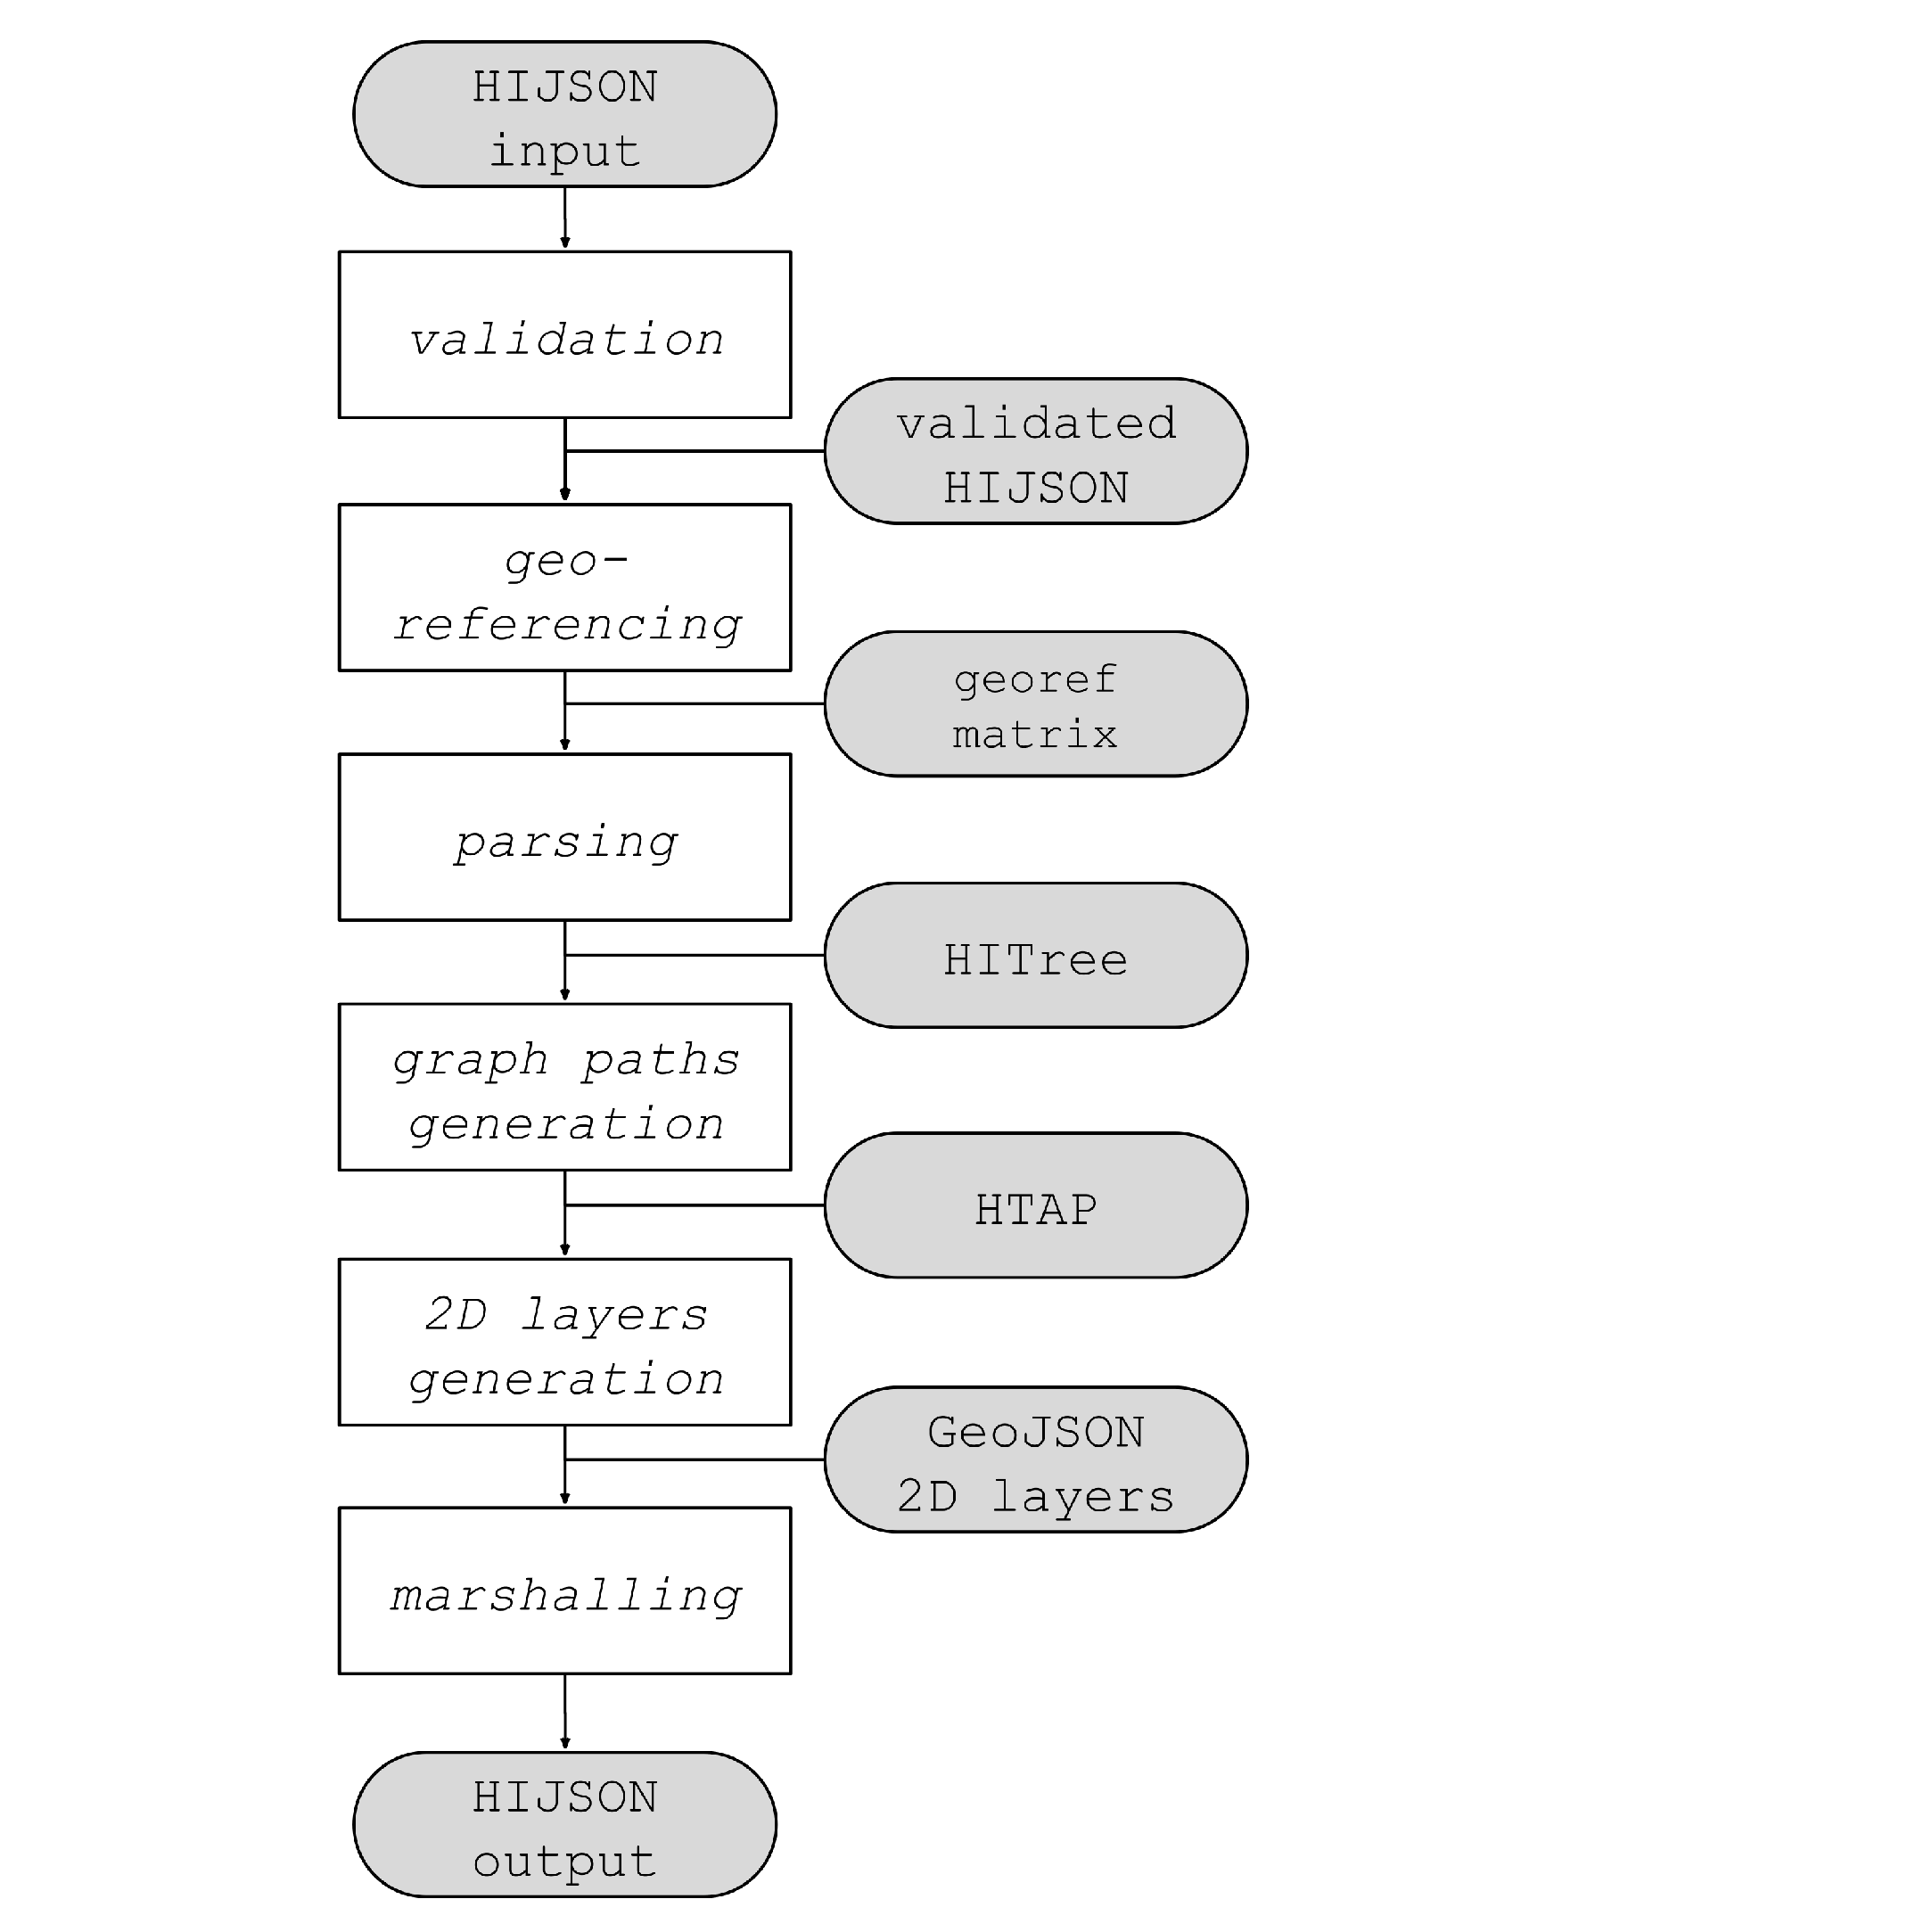
\epsfig{file=images/pipeline.eps, height=0.4\textwidth}
\caption{HIJSON processing pipeline}
\label{fig:pipeline}
\end{figure}

\begin{enumerate}
\def\labelenumi{\arabic{enumi}.}
\itemsep1pt\parskip0pt\parsep0pt
\item
 \textit{\texttt{validation}} - The first one is the validation stage. In
  order to begin with the effective transformations the input HIJSON  document
  must be compliant with both the syntax format and the structural requirements.   In the
  case the validation stage fails, processing aborts and does not continue to
  following stages; intead if this stage successes, then the output for the next stage is a
  validated  HIJSON.

\item
 \textit{\texttt{georeferencing}} - In the second stage, in order to allow
 for continuous outdoor/indoor navigation, the system needs to compute
 the georeferencing matrix, a linear operator able to transform local
 coordinates into global coordinates (world coordinate
 system --- latitude and longitude angles) and vice versa. This task is
 accomplished by solving a linear system obtained from information
 contained in HIJSON configuration part and precisely from the
 correspondence of three real world points to three points included
 into the HIJSON document.
\item
 \textit{\texttt{parsing}} - The parsing stage takes the validated and
 georeferenced HIJSON as its input, that as illustrated before can be
 thought of as a list of HIJSON Elements, parses them and produces an
 instance of the HIJSON Tree. The HIJSON Tree is an object in memory
 representing the hierarchical structure of the building described
 by the HIJSON document.
\item
 \textit{\texttt{graph of paths generation}} - The fourth stage is in char\-ge
 of the generation of the graph of paths. The algorithm to achieve such a 
 goal is introduced in Section~\ref{sec:paths}. The graph of paths can be used to compute valid directions between pairs of points of
 interest inside the building model. Once the graph of paths has been computed, the
 input HIJSON Tree is augmented with paths information, becoming what
 has been called an HTAP (HIJSON Tree Augmented with Paths).
 Augmentation always takes place in the form of an addition of leaf nodes as children of a
 specific element (e.g. ``room'').
\item
 \textit{\texttt{2D layers generation}} - The fifth stage concerns the
 generation of GeoJSON \emph{layers}. For each storey of the building, the Toolkit generates a
 GeoJSON layer that can be used for the creation of a 2D map. Each layer
 contains only the children of a `level' node of the HIJSON Tree. 
 The presence of a specific element inside the layer can be finely tuned 
 by means of a Boolean value. The geographical coordinates of every elements
 are calculated by a series of multiplications between transformation matrixes obtained 
 during the tree traversal to the local coordinates.
\item
 \textit{\texttt{marshalling}} - The last stage is responsible for executing
 a serialization of the the transformed data. This stage, in which are performed tasks like breaking
 dependency-loops and stringification, is
 mainly useful  server-side, as the output is there stored ready to be
 served to any requiring client.
\end{enumerate}

\subsubsection{Automatic generation of valid paths}\label{algorithmics-automatic-generation-of-valid-paths}\label{sec:paths}

The fourth stage of the processing pipeline is responsible for the
generation of a graph of valid paths through the entire model
represented by the input HIJSON document. The graph generated according
to the algorithm described in the following, although non optimal,
ensures a complete coverage of the surface while limiting the number of
generated nodes. The resulting graph is weighted on the edges with nodes
distances. Each graph node may represent either:

\begin{enumerate}
\def\labelenumi{\alph{enumi}.}
\itemsep1pt\parskip0pt\parsep0pt
\item
 a \emph{standard path node}, i.e.~a junction node or possibly an endpoint of a
 path;
\item
 a \emph{connection node}, used as subproblem composing element in the divide et
 impera approach adopted;
\item
an \emph{element node} i.e.~HIJSON Element (whose HIJSON Class explicitly grants
 his presence in the graph), typically an endpoint of a path.
\end{enumerate}

The graph of paths allows for calculations of directions between any two given
nodes. Although different approaches have been explored \cite{6999103}, 
a very classical solution has been selected in this case, so directions 
are actually computed client-side by applying the Dijkstra algorithm to the graph. 

Taking advantage of the hierarchical structure of the HIJSON document,
and according to the divide et impera approach, the problem of 
paths generation is split in several sub-problems, which consist in
the computation of the sub-graphs relative to each individual space, more generally a single room. The sub-graphs are then linked together through the
connection nodes (which in most cases represent doors). The resolution
of each sub-problem (as depicted in Figure~\ref{fig:graph-generation}), 
is composed by four steps, as detailed below.

\begin{enumerate}
\def\labelenumi{\arabic{enumi}.}
\itemsep1pt\parskip0pt\parsep0pt
\item
 Computation of the walkable area of the space: this task is
 accomplished by subtracting the shape of the obstacles from the area
 of the space; the result is typically a surface with holes.
\item
 Triangulation of the walkable area: the computed surface is
 triangulated taking into account the presence of holes.
\item
 Identification of graph nodes: for each triangle side completely
 internal to the area, its midpoint is selected as standard path node.
\item
 Junction of nodes: nodes relative to the same triangle are then linked
 pairwise; both element nodes and connection nodes (i.e.~doors) are
 linked to the nearest node of the space (i.e.~room).
\end{enumerate}

\begin{figure*}[!htbp]
 \centering
 \begin{subfigure}[b]{0.235\textwidth}
 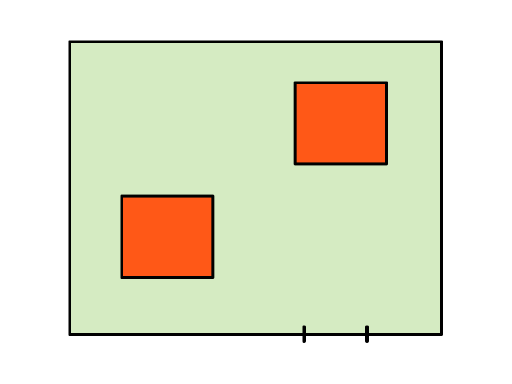
\includegraphics[width=\textwidth]{images/graph-generation/single/graph-generation-1}
 \caption{}
 \label{fig:graph-generation-a}
 \end{subfigure}
 ~
 \begin{subfigure}[b]{0.235\textwidth}
 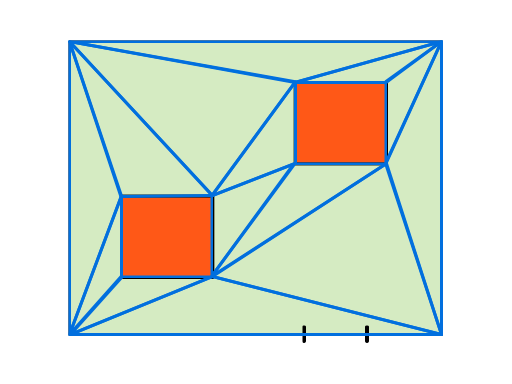
\includegraphics[width=\textwidth]{images/graph-generation/single/graph-generation-2}
 \caption{}
 \label{fig:graph-generation-b}
 \end{subfigure}
 ~
 \begin{subfigure}[b]{0.235\textwidth}
 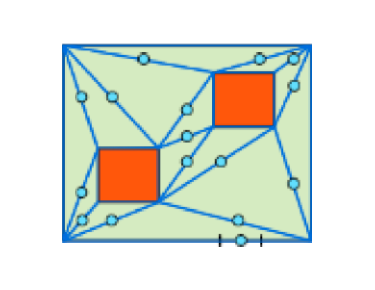
\includegraphics[width=\textwidth]{images/graph-generation/single/graph-generation-3}
 \caption{}
 \label{fig:graph-generation-c}
 \end{subfigure}
 ~
 \begin{subfigure}[b]{0.235\textwidth}
 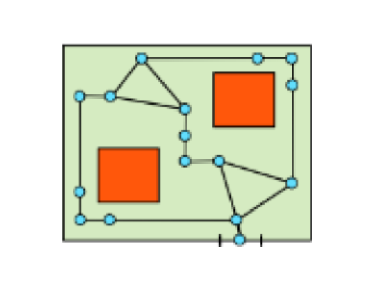
\includegraphics[width=\textwidth]{images/graph-generation/single/graph-generation-4}
 \caption{}
 \label{fig:graph-generation-d}
 \end{subfigure}
 
 \caption{graph of paths generation: 
 (a) detection of obstacles and computation of walkable area; 
 (b) triangulation of walkable area; 
 (c) identification of graph nodes; 
 (d) junction of nodes.
 }
 \label{fig:graph-generation}
\end{figure*}

\subsection{HIJSON Class definition}\label{hijson-class-definition}

To make better use of the possibilities offered by the HIJSON Toolkit and by the
HIJSON document format, some custom dynamic behaviors can be described. These
behaviors encapsulate the specificities relative to communication
protocols with the sensors, as well as to features of user interaction. The
interface for such behavior is the HIJSON Class.

\begin{figure}[!h]
\centering
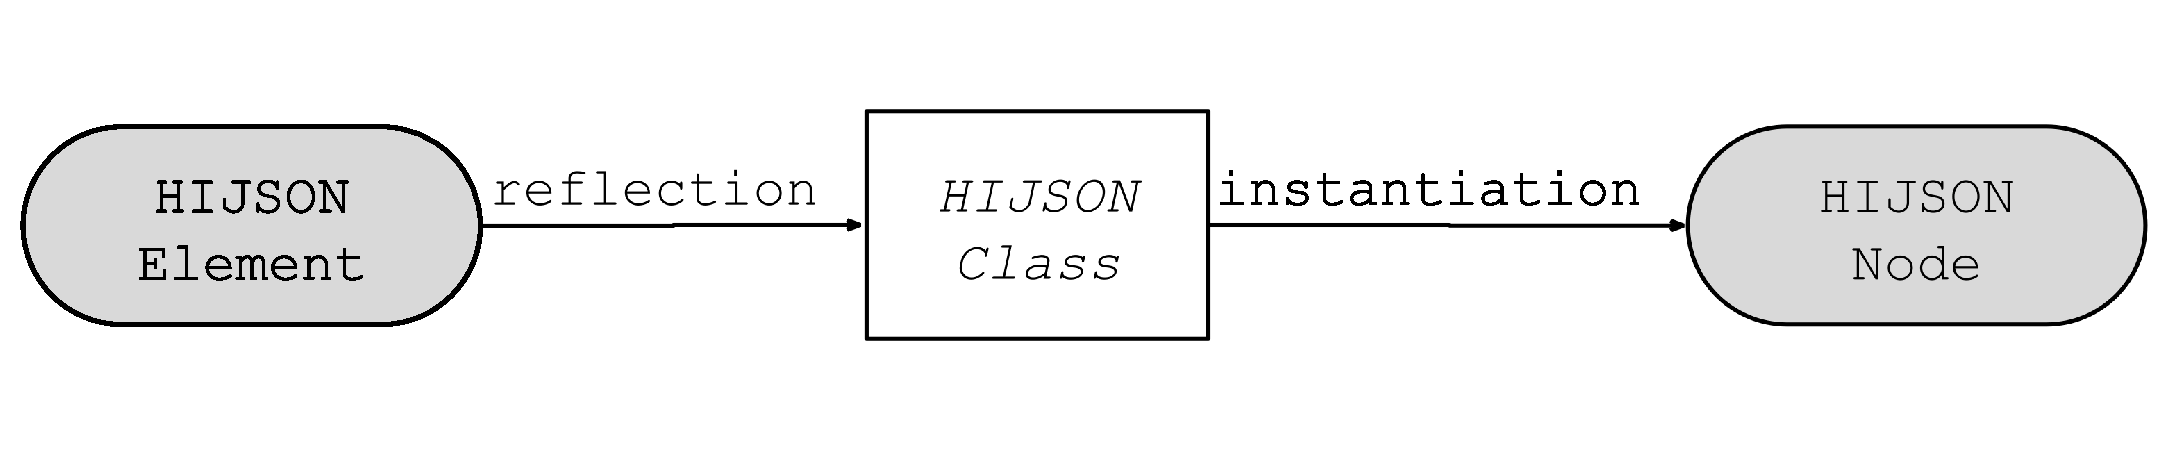
\epsfig{file=images/element-class-node.eps, width=0.44\textwidth}
\caption{HIJSON Element/Class/Node relashionship}
\label{fig:elem-class-node-rel}
\end{figure}

Every HIJSON Element of the input HIJSON document has a dynamic
counterpart, a running instance called \emph{HIJSON Node}, instantiated
according to the corresponding HIJSON Class via reflection methods (see
Figure~\ref{fig:elem-class-node-rel}).

To specify a new \emph{HIJSON Class} means to extend the Toolkit to deal with a
new class of HIJSON Element.
To extend the toolkit in order to deal with a new class of HIJSON Element is
required to specify a new HIJSON Class, by defining the following
properties and methods:

\begin{itemize}
\item
 \texttt{in\_graph}: a Boolean value to express if the element is an
 approachable point in the graph of paths;
\item
 \texttt{in\_2D\_map}: a Boolean value to express if the element must 
 be shown in the 2D map;
\item
 \texttt{get2DStyle()}: a method that returns the 2D map appearance of
 the element, essentially HTML and CSS code;
\item
 \texttt{get3DModel()}: a method that returns the 3D model appearance of
 the element, i.e.~an instance of \texttt{Obj\-ect\-3D} of the \emph{THREE.js} 
 framework;
\item
 \texttt{getWidget()}: a method that returns the information widget, a
 \emph{React} component;
\item
 \texttt{getProxy()}: a method that returns the server-side proxy which
 encapsulate the IoT sensor communication protocol, i.e.~a \emph{Node.js}
 module.
\end{itemize}

User's needs for new indoor elements, greatly different sensor equipments,
alternative representations of 2D or 3D viewports are accepted by the
definition of new HIJSON Classes, that so provide single-point
custom extensions of the Toolkit capabilities.


\begin{figure*}[htb]
\centering
% 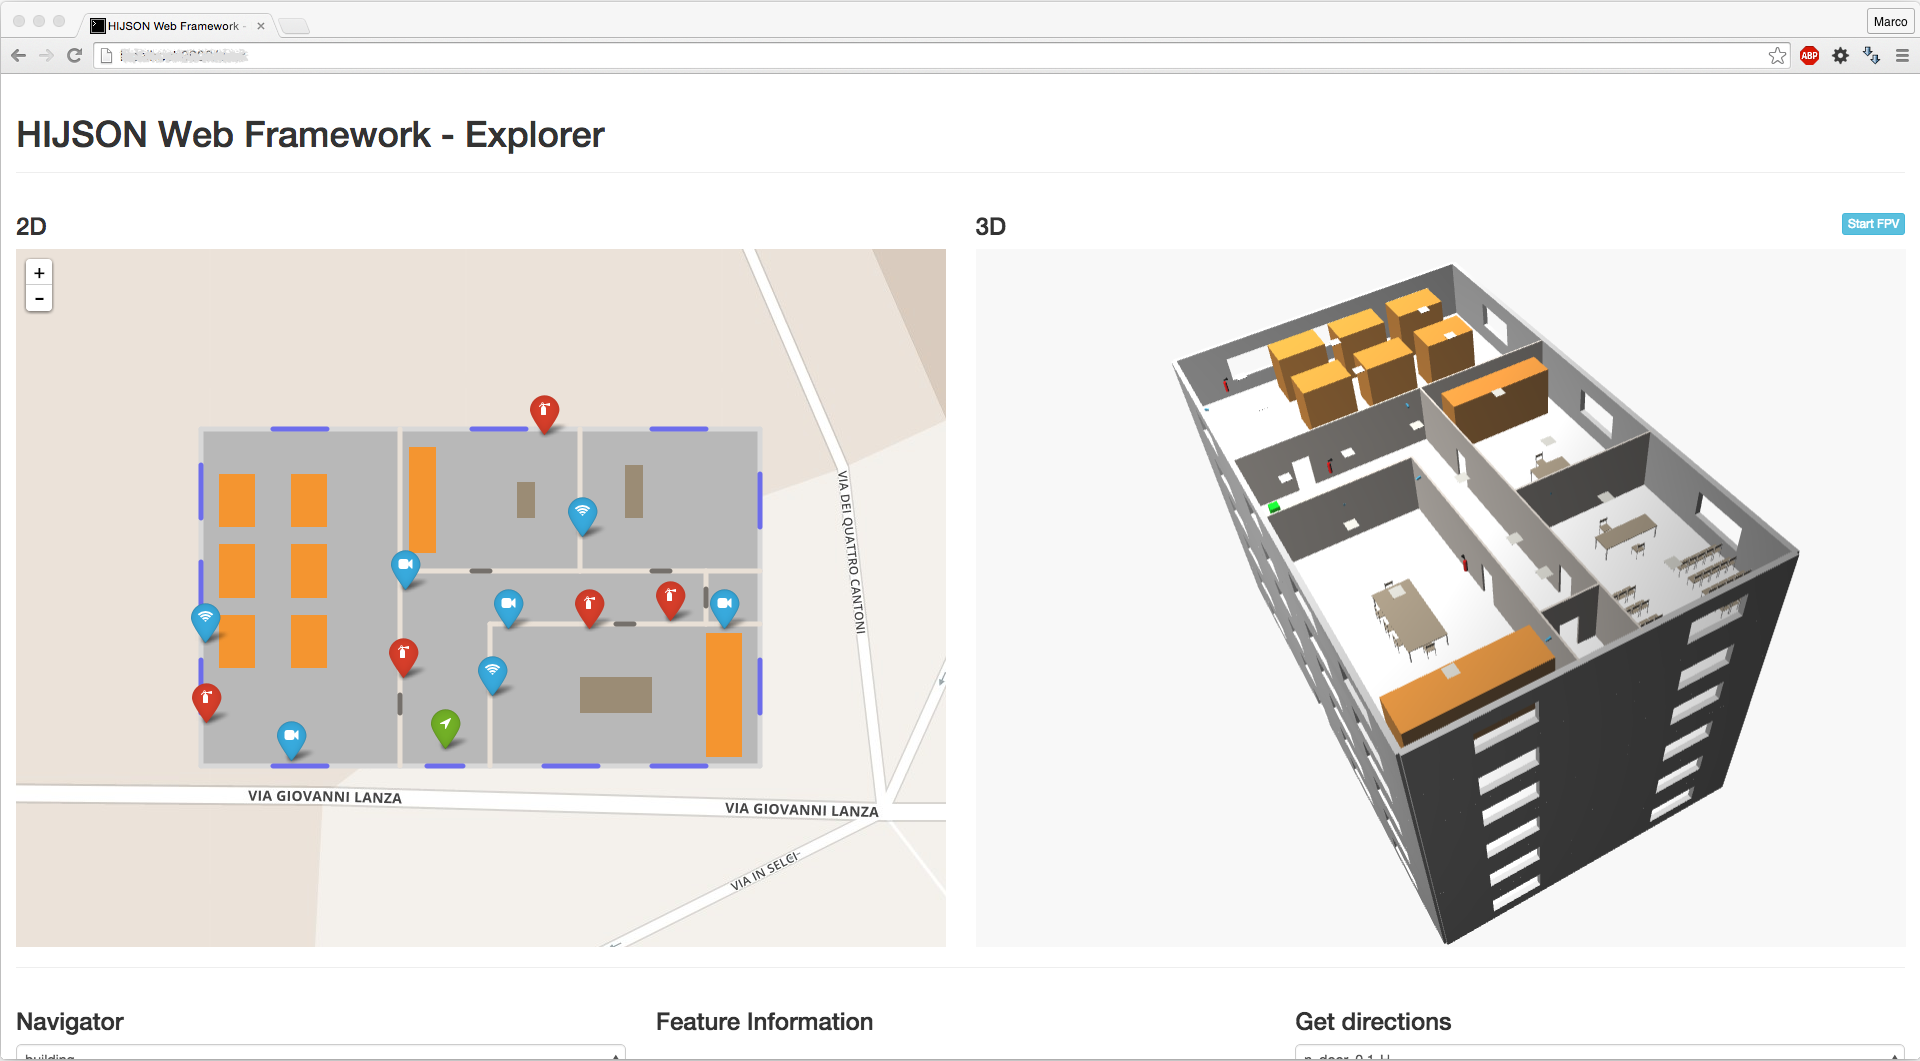
\includegraphics[width=\textwidth]{images/web_framework_1.png}
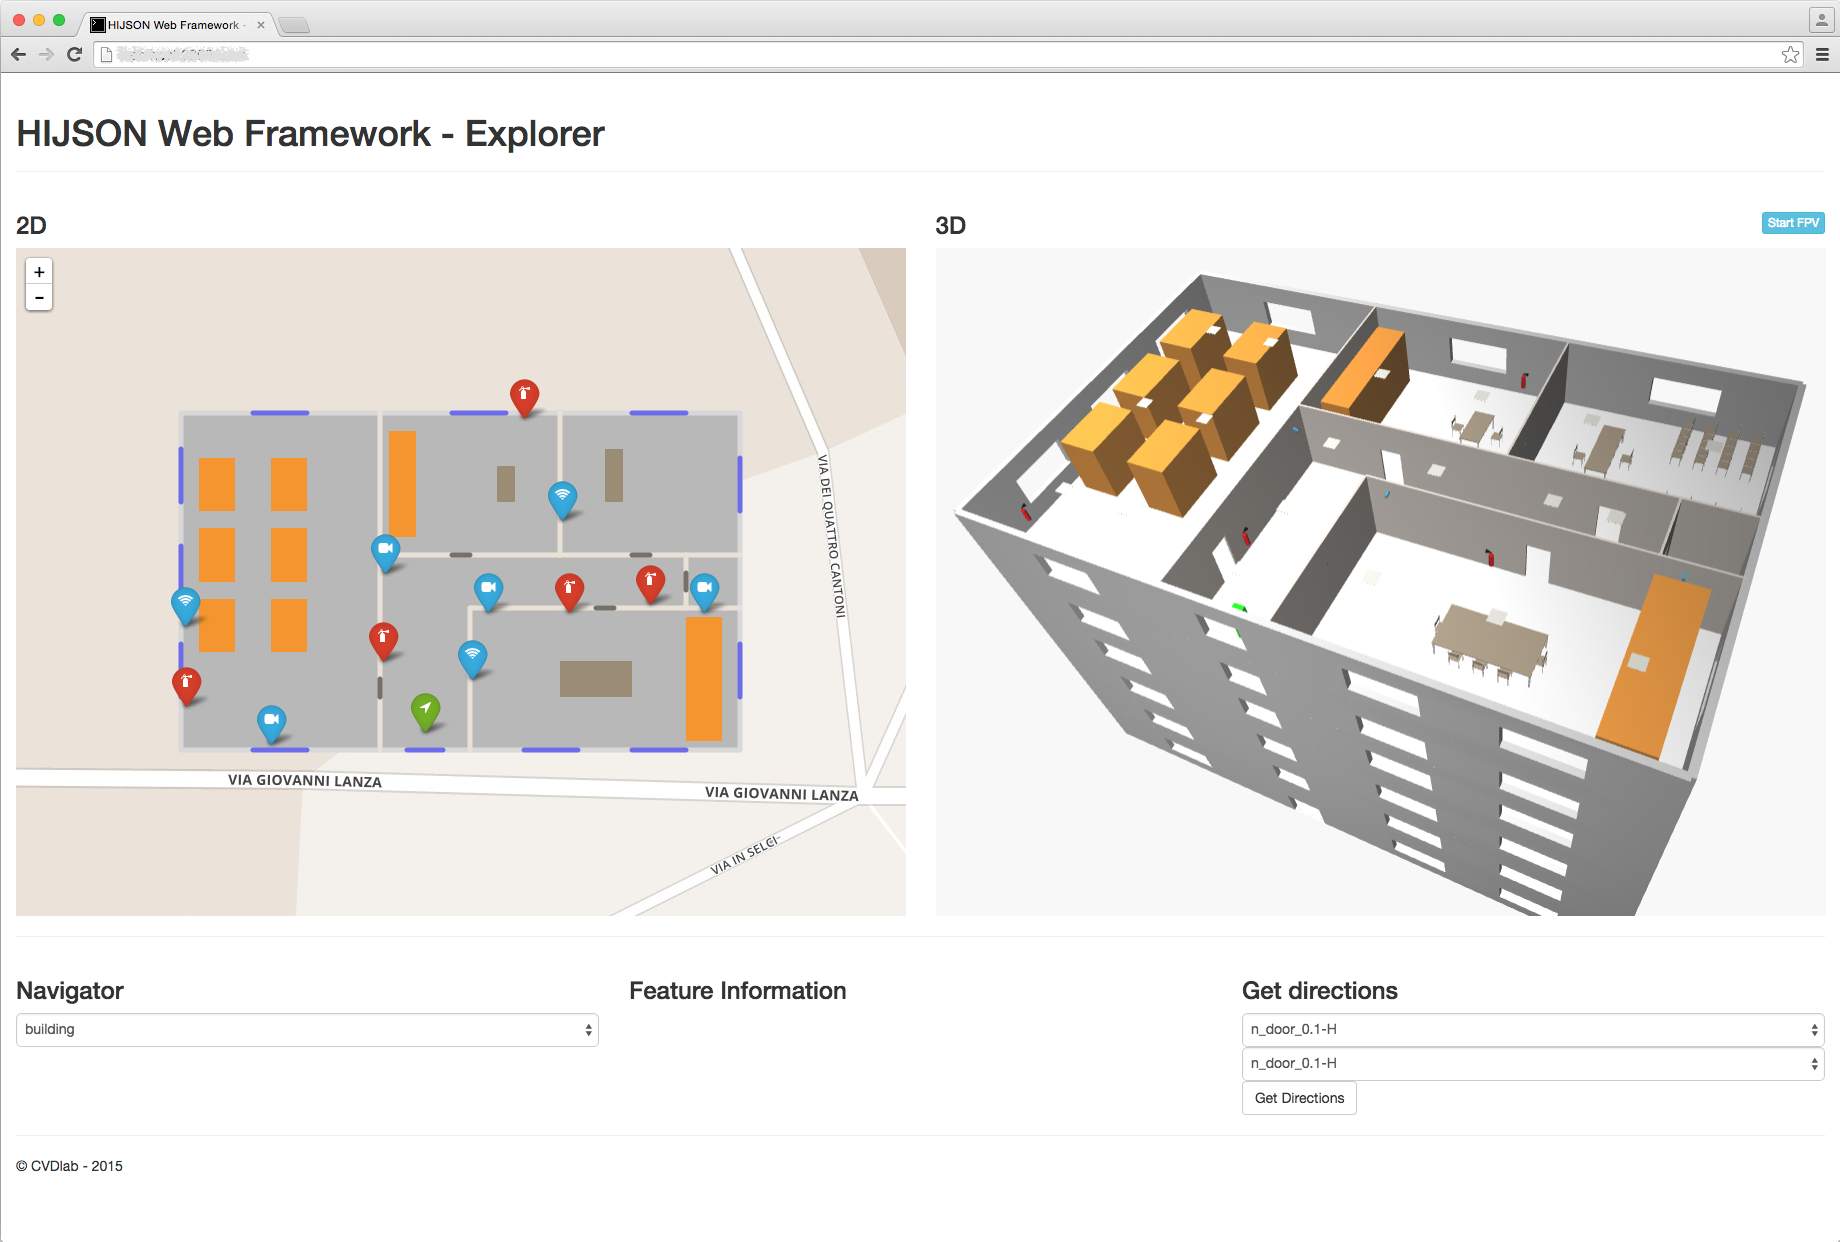
\includegraphics[width=\textwidth]{images/web_framework_2.png}
\caption{HIJSON Web Framework UI}
\label{fig:web-framework-ui}
\end{figure*}


\section{HJSON Web Framework}\label{hjson-web-framework}

The HIJSON Web Framework responds to the needs of an extendable,
customizable, and scalable web framework which provides at the same time IoT
monitoring, realtime multi-person tracking and cross-floor user
navigation.

Expandability and customizability derive from both design choises and
HIJSON inherent characteristics, i.e.~the possibility of semantic extensions.
Scalablility is directly borrowed from technologies used for the
software development: \emph{JavaScript} language, using \emph{Node.js},
in particular \emph{Express.js} as backend framework, exploiting the
power of WebSocket protocol through the \emph{Socket.io} library.

Being supported by the \emph{web-as-a-platform}, the framework exposes
also an high availability: it is so simple to use as to visit a
website, both from desktop or mobile devices, without explicit
requirements to install any software package from proprietary stores---access to
which is often denied from business devices.

The HIJSON Web Framework deeply relies on HIJSON Toolkit and offers an
all-inclusive client/server architecture and a convenient and highly interactive
user interface, leaving aside the specific indoor positioning system and
the IoT sensors to deal with. A robust application interface is provided and
described in the following section.

\subsection{Applications}\label{applications}

The Framework has been designed with focus on two different kind of
users: the \emph{Explorer} and the \emph{Supervisor}. They have
different requirements and are likely equipped with different devices:
while the \emph{Supervisor} monitors the indoor environment through a
desktop workstation, the \emph{Explorer} has a smartphone available and
needs to be routed across the building.

In both cases, the web platform ensures a perfect alignment with the
BYOD (Bring Your Own Device) approach, nowadays often supported by companies
that encourage employees to use personal devices.

\begin{figure*}[htb]
\centering
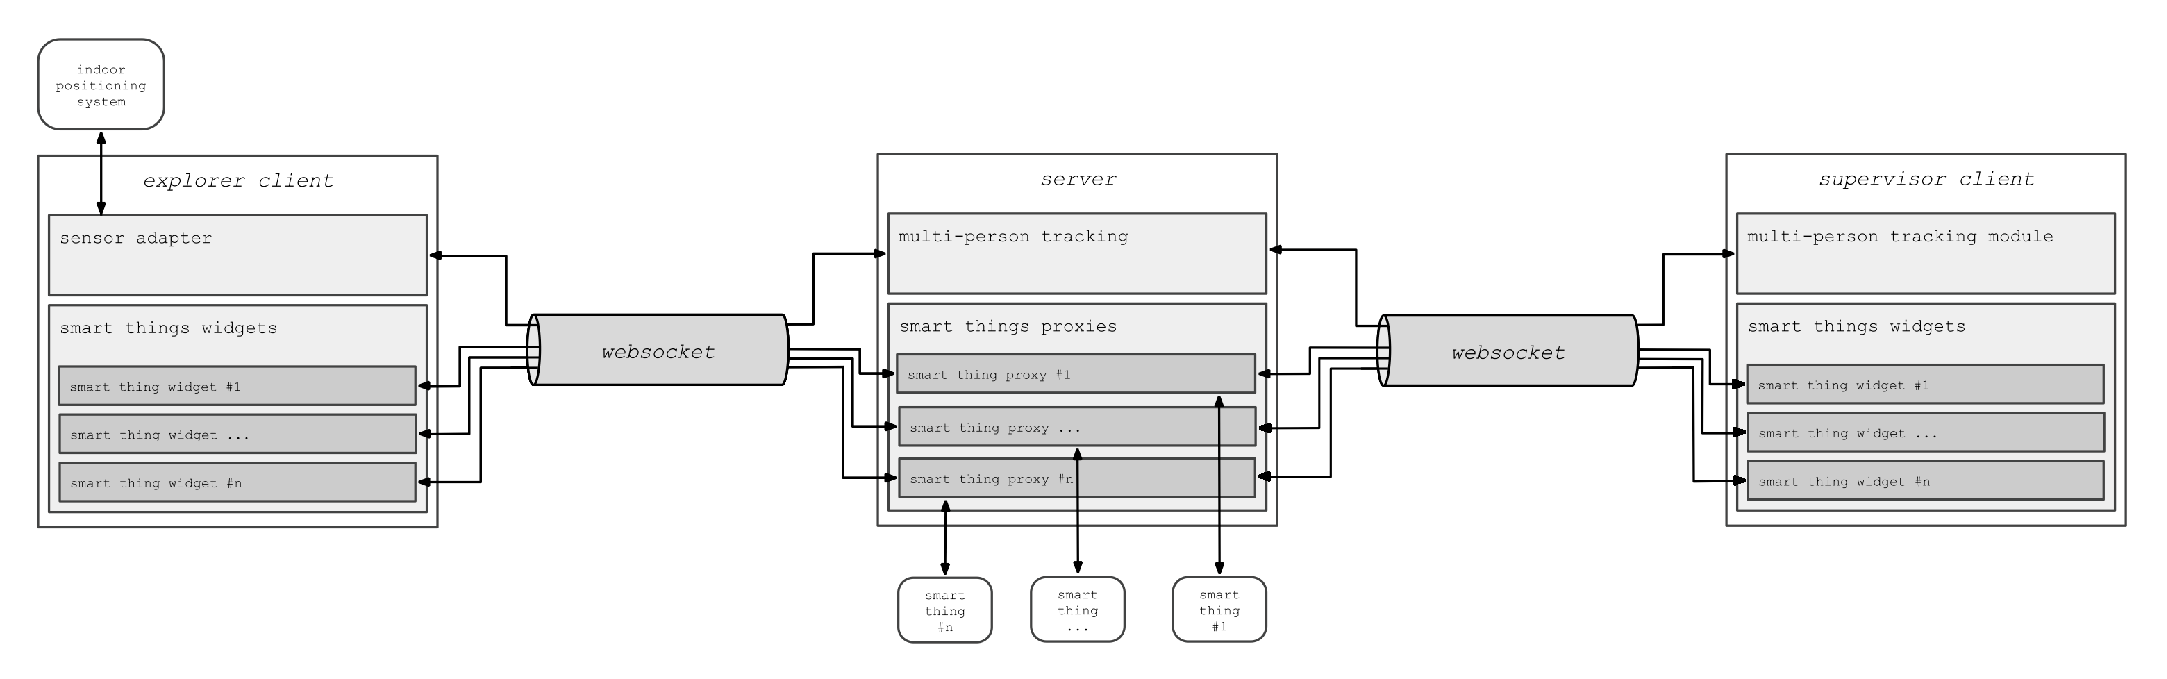
\epsfig{file=images/architecture.eps, width=\textwidth}
\caption{HIJSON Web Toolkit architecture}
\label{fig:architecture}
\end{figure*}


\subsubsection{IoT monitoring}\label{iot-monitoring}

An \emph{IoT monitoring application} consists of an interface showing the user, in a single, integrated and centralized way, the information collected from all the smart objects modelled in the HIJSON document.
It is proper of IoT monitors to provide bidirectional communication, since the interface lets the user have information coming from smart objects, but also allows him to send commands to them. 

As the name itself may suggest, it is an activity specifically performed by a \emph{Supervisor} user, but it can be also suitable to be deployed for the \emph{Explorer} user, since she can take advantage of the interactive information coming from the surroundings objects while she moves across the indoor environment.

Monitoring different smart objects may require different ways to visualize and/or send data and commands.
Modularity and extendibility of the application respond superbly to these requirements, by providing for each class of objects a different interface of visualization and interaction, as a result of the information hiding and incapsulation principles introduced by the HIJSON Class.
In particular, the user interface is characterized by a dual-display mode, that allows the user to see at the same time a 2D map that gives an overall glance in a simplified plan, and a 3D virtual environment to navigate into, as shown in Figure~\ref{fig:web-framework-ui}.

Alongside with typical smart objects, suitable to deal with like thermostats, where the user can read the room  temperature and turn the heating on/off, other kinds of objects that are not properly considered ``smart'' can be integrated into the HIJSON environment. It is the case, for example, of fire estinguishers, that are able to show the date of their last check, stored in a database.

\subsubsection{Realtime multi-person tracking}\label{realtime-multi-person-tracking}

Real=time multi-person tracking allows a \emph{Supervisor} to monitor the current
real position of people inside the building. This kind of task can be useful for
several reasons, including security, logistics or to supervise composite operative
workflows. Each device equipped with the \emph{Explorer} application is in charge of locating
itself, interacting with the indoor positiong saystem, and notifying the current
position in continuos mode. Evidence of the people position is given to the
\emph{Supervisor} both into a 2D map and an immersive 3D virtual environment (see Figure~\ref{fig:web-framework-ui}).

\subsubsection{Cross-storey user navigation}\label{cross-storey-user-navigation}

The HIJSON Framework also provides the capability to give directions to
\emph{Explorer} users that must move across the indoor environment. The
user specifies a starting and an ending point and the system provides him with
a valid and optimal connection path. This feature
strongly rely on the graph of paths generated by the Toolkit, so starting and
ending points must be nodes of the graph. \emph{Connection nodes} are introduced to
represent stairs or elevators, enabling cross-storey paths to be computed.
Since paths can span more than one storey, the most effective way
to display them to the user is to show the connection nodes merged in more than one 2D map.

\subsection{Architecture}\label{architecture}

Like the vast majority of the web based applications, the Framework exposes an
overall architecture that is inherently \emph{client/server}. In particular,
two different types of possible client are identifiable, one for each different 
kind of users: the \emph{Supervisor} client and the \emph{Explorer} client. 
Both of them connect to the same server.

The indoor space described by the input HIJSON document is
processed by the server via the processing pipeline. After that, any connecting
\emph{Explorer} client, presumably via a mobile device, will be provided
with the information to perform cross-storey navigation of the building, while
reporting the user position to the server. The server will feed any connecting
\emph{Supervisor} client with users positions, along with data from sensor-
equipped objects present in the environment, achieving both IoT monitoring and 
realtime multi-person tracking.

\subsubsection{Server Architecture}\label{server-architecture}

An architectural scheme of the framework is provided in Figure~\ref{fig:architecture}. A web server module is responsible for listening to
connecting clients. Each client connection is handled by the web server module
providing all the required resources by opening a websocket channel, in order to
have both \emph{Explorer} and/or \emph{Supervisor} communication
protocol data flow within. In particular, the \texttt{multi-person\ tracking} module receives
position data from \emph{Explorer} clients. It aggregates and sends these
information to connected \emph{Supervisor} clients through the websocket
channel, using a simple but reliable protocol described later. Indipendence
from particular IoT sensor equipment communication protocols is achieved
introducing a \texttt{smart\ object\ proxy} module. This one is defined in the HIJSON Class
and is obtained via the {\tt getProxy()} method for each smart
object modelled as previously described).

\subsubsection{Explorer client architecture}\label{explorer-client-architecture}

The \emph{Explorer} client architecture is generally deployed on a mobile
device, which is usually supplied to a user who needs to be routed across the
environment described by the HIJSON document. The {\tt sensor\ adapter} module
encapsulates the communication logic with the indoor positioning system. The
presence of this module ensures indipendece from particular tecnologies, so
allowing the \emph{Explorer} client to rely on different indoor positioning
systems (WiFi, LTE, etc.).

Every time a {\tt sensor\ adapter} observes a perceptible
modification in user position, sends the new position information to the
server through the single opened websocket, spawning a simple message with the
following syntax:

\begin{verbatim}
currentPosition = {
 coordinates: [x, y],
 levelId: level-ID 
}
\end{verbatim}

Relevant information includes, beside current coordinates, the indication of
the storey of the possibly multilevel building the user is in.

It is to remark that, when not outflanked by the introduction of an external
server, the problem of communication between positioning system and the low
level APIs of the browser is left to positioning system itself or to whom is
in charge of specific deployments of the HIJSON Web Framework.
The \texttt{smart\ object\ widget} module, being in common with the
client \emph{Supervisor}, will be discussed in the next section.

\subsubsection{Supervisor client architecture}\label{supervisor-client-architecture}

The architecture of \emph{Supervisor} client includes two modules. The first
one, named {\tt multi-person\ tracking} module, is responsible to
receive through the websocket, from the server information about
\emph{explorers} of the environment, showing them in the user interface. The
second module, named {\tt smart\ object\ widget}, communicates with the
server to propose the user realtime information about sensor-equip\-ped
objects in the environment. Data passes through the single websocket
opened between the server and every \emph{Supervisor} Client. Relying on a
naive but effective communication protocol, each {\tt smart object widget}
exchanges data only with its corresponding {\tt smart object proxy} on the server. To
ensure the data are posted only when the user requires the information
relative to a specific smart object, a \emph{widget lifecycle protocol} is
implemented. This one is based on 4 event triggers {\tt on\_before\_show},
{\tt on\_show}, {\tt on\_before\_hide}, {\tt on\_hide}, as suggested by their names.
When the user requires information about a smart object, its widget has
to be rendered, and {\tt on\_before\_show} the server is notified to
connect via relative proxy to the sensor. Once connected, the server
begin to send data via websocket. Received data are shown through the
widget to the user. When done, the {\tt on\_before\_hide} event of the
widget is triggered, a notification is sent to the server announcing to stop sending
data, and the proxy closes the connection to the sensor. Widget lifecycle
protocol ensures that only required data are sent from the server to the
client.


\section{Case study}\label{case-study}

As case study of the discussed approach, we have taken into account the need of Sogei S.p.A. to support its maintenance service  workflow, since the data center, one of biggest data centers in Europe, is subject to very strict access control policies. 

The overal state of the data center can be monitored through the \emph{Supervisor} client. In this case the considered smart objects belong to a range of different devices, going from webcams, that provide on request the captured video streams, by way of alarm and antifire systems, till to individual servers, that can be monitored along several dimensions, including operating temperature, workload, etc. 

The most common maintenance scenario consists of a intervention by a technician that have to move across the environment, and locate within a huge data center the machine on which to operate, a not trivial task due to the presence of thousands of similar-looking machine racks. Thus the operator will be equipped with an \emph{Explorer} client, which will drive him to the target machine on which operate, while continuously notifying to a security \emph{Supervisor} his position, obtained by interacting with the indoor positioning system.
The mantainance workflow supervisor, using the \emph{Supervisor} client, is able to monitor the operator position within the data center, verifying that he does not deviate on unauthorized paths, triggering some console alarm if this happens.

The purpose is to support  the process of those in charge of carrying out the ``ticket-maintenance'' activities, as quickly  as possible and without error. The ``maintenance man'' will be guided to the right sub-system among thousands of racks. The real-time awareness of the relative positions between the 'maintenance man' and the rack ---containing the sub-system---will help us to reduce intervention times and to increase safety. By  knowing when the maintenance process starts, the system  can automatically move, in real time, services, which are hosted on virtual machines, to other systems, thus maintaining the continuity of services and, at the same time,  reducing  the global risk factor. When the ``ticket-maint\-enan\-ce'' is over, and the technician goes away, it is possible to immediately  restore  the pre-existing conditions of services after a complete test has been performed.




%----------------------------------------------------------------------------

% right sub­system (inside the rightrack among thousands). We will call them the
% ``maintenance man''. The real­time awareness of the relative positions between
% the ``maintenance man' andthe rack ­ containing the sub­system ­ will help us
% reducing intervention times and increasing safety. If you knew when the
% maintenance process starts, you couldautomatically move,in real time,
% services, that is virtual machines, to other systems,thus
% maintainingcontinuity of services and, in the same time, reducing the
% globalrisk factor. Whenmaintenance is over, and the technician moves away, you
% couldinstantly restore thepre­existing conditions of services, that is,
% immediately after havingperformed an outright test.

% We are now trying to
% verify the possibility to perform a realtime control over the maintenance
% workflow in a complex Data Center. 

% Inparticular, wehave to support the process of those in charge of carrying out
% the ticket­maintenance reaching, as quick as possible and without error, the
% right sub­system (inside the rightrack among thousands). We will call them the
% ``maintenance man''. The real­time awareness of the relative positions between
% the ``maintenance man' andthe rack ­ containing the sub­system ­ will help us
% reducing intervention times and increasing safety. If you knew when the
% maintenance process starts, you couldautomatically move,in real time,
% services, that is virtual machines, to other systems,thus
% maintainingcontinuity of services and, in the same time, reducing the
% globalrisk factor. Whenmaintenance is over, and the technician moves away, you
% couldinstantly restore thepre­existing conditions of services, that is,
% immediately after havingperformed anoutright test.



\section{Conclusions}\label{conclusions}

In this paper a novel format for indoor cartographical description has been introduced, named HIJSON. Utilization of local metric coordinate system, avoiding the manipulation of geographical coordinate really inconvenient when dealing with indoor spaces and objects, greatly simplify the drawing up process of the document. Process that can be further improved realizing a graphical editor to assist the user during the description of the indoor space. The implementation of such an editor is already programmed.

The HIJSON format focuses on a hierarchical representation of the indoor spaces that allows for completely capturing their topology. On the basis of this representation a virtual web environment can be rebuilt working as a unifying platform to run a bunch of different applications. The reference architecture of such a platform has been also implemented and described in this work. The architecture supports a range of applications: IoT monitoring, realtime-multiperson tracking and user crossfloor navigation are already implemented and described. A very convenient way to extend representation capabilities of smart objects is also mentioned as semantic extensions. These extensions (which affects both document format and web framework) might be easly collected in a public repository. Community could both use public available extensions or contribute by mapping new (smart) objects inside the HIJSON document.


%
% The following two commands are all you need in the
% initial runs of your .tex file to
% produce the bibliography for the citations in your paper.
\bibliographystyle{abbrv}
\bibliography{doceng2015.bib} % doceng2015.bib is the name of the Bibliography in this case
% You must have a proper ".bib" file
% and remember to run:
% latex bibtex latex latex
% to resolve all references
%
% ACM needs 'a single self-contained file'!
%
%\balancecolumns
\end{document}
